\documentclass[10pt]{report}

\usepackage{amsmath}
\usepackage{amssymb}
\usepackage{graphicx}
\usepackage{helvet}

\setlength{\paperheight}{3in}
\setlength{\paperwidth}{4in}
\pdfpagewidth=\paperwidth
\pdfpageheight=\paperheight

\setlength{\textwidth}{3.75in}
\setlength{\textheight}{2.5in}

\setlength{\oddsidemargin}{-1.0in}
\setlength{\evensidemargin}{-1.0in}
\setlength{\topmargin}{-1.25in}

\newcommand{\sld}[1]{\newpage{\noindent\Large \ \ \ \underline{#1}}\vspace*{8pt}}
\newcommand{\spc}{\hspace*{0.25in}}

\newcounter{gmlrx}
\newcounter{gmlry}
\newcommand{\gmnode}[3]{\put(#1,#2){\circle{20}}\put(#1,#2){\makebox(0,0){$#3$}}}
\newcommand{\gmplate}[5]{
\setcounter{gmlrx}{#1}\addtocounter{gmlrx}{#3}
\setcounter{gmlry}{#2}\addtocounter{gmlry}{-#4}
\put(#1,#2){\line(1,0){#3}}
\put(#1,#2){\line(0,-1){#4}}
\put(\value{gmlrx},\value{gmlry}){\line(-1,0){#3}}
\put(\value{gmlrx},\value{gmlry}){\line(0,1){#4}}
\setcounter{gmlrx}{#1}\addtocounter{gmlrx}{5}
\setcounter{gmlry}{#2}\addtocounter{gmlry}{-6}
\put(\value{gmlrx},\value{gmlry}){\makebox(0,0){$#5$}}
}

\newcommand{\mypart}[1]{\newpage\vspace*{36pt}\noindent\ \ \ \ {\huge #1}}


\begin{document}
\sf%
\vspace*{18pt}
\noindent
\spc{\huge Models of Annotation (II)}
\\[24pt]
\spc{\large Bob Carpenter,} \ \ {\it LingPipe, Inc.}
\\[8pt]
\spc{\large Massimo Poesio,} \ \ {\it Uni.\ Trento}
\\[48pt]
\spc LREC 2010 (Malta)

\mypart{Mechanical Turk Examples}
\vfill
(Carpenter, Jamison and Baldwin, 2008)

\sld{Amazon's Mechanical Turk}
\begin{itemize}
\item ``Crowdsourcing'' Data Collection (Artificial AI)
\item We provide web forms to Turkers (through REST API)
\item We may give Turkers a qualifying/training test
\item Turkers choose tasks to complete
\begin{itemize}
\footnotesize
\item We have no control on assignment of tasks
\item Different numbers of annotations per annotator
\end{itemize}
\item Turkers fill out a form per task and submit
\item We pay Turkers through Amazon
\item We get results from Amazon in a CSV spreadsheet
\end{itemize}


\sld{Case 1: Named Entities}

\includegraphics[width=0.95\textwidth]{pngs/big-ne-form.png}


\sld{Named Entities Worked}

\begin{itemize}
\item Conveying the coding standard
\begin{itemize}
\footnotesize
\item official MUC-6 standard dozens of pages
\item examples are key
\end{itemize}

\item Fitts's Law
\begin{itemize}
\footnotesize
\item time to position cursor inversely proportional to target size
\item highlighting text: fine position + drag + position
\item pulldown menus for type: position + pulldown + select
\item checkboxes for entity at a time: fat target click
\end{itemize}
\end{itemize}

\sld{Discussion: Named Entities}

\vspace*{-6pt}
\begin{itemize}
\item 190K tokens, 64K capitalized, 4K person name tokens
\begin{itemize}
\footnotesize
\item 4K / 190K = 2.1\% prevalence of entity tokens
\end{itemize}
\item 10 annotators per token
\item 100+ annotators, varying numbers of annotations
\item Less than a week at 2 cents/400 tokens (US\$95)
\item Aggregated Turkers better than LDC data
\begin{itemize}
\footnotesize
\item Correctly Rejected:
{\tt\footnotesize Webster's, Seagram, Du Pont,
\\
Buick-Cadillac, Moon, erstwhile Phineas Foggs}
\item Incorrectly Accepted: {\tt\footnotesize Tass}
\item Missed Punctuation: {\tt\footnotesize J~E.~``Buster'' Brown}
\end{itemize}

\end{itemize}


\sld{Case 2: Morphological Stemming}

\includegraphics[width=0.95\textwidth]{pngs/stems-v4.png}

\sld{Morphological Stemming Worked}

\begin{itemize}
\vspace*{-8pt}
\item Coded and tested by intern (Emily Jamison of OSU)
\begin{itemize}
\footnotesize
\item Less than one month to code, modify and collect 
\end{itemize}
\item Three iterations of coding standard, Four of instructions
\begin{itemize}
\footnotesize
\item began with full morphological segmentation (too hard)
\item simplified task to one stem with full base (more ``natural'')
\item added previously confusing examples and sample affixes
\end{itemize}

\item Added qualifying test

\item 60K (50K frequent Gigaword, 10K random) tokens
\item 5 annotators / token
\end{itemize}





\mypart{Generative Labeling Model}
\vfill
\noindent
\ \ \ \ (Dawid and Skene 1979; Bruce and Wiebe 1999)

\sld{Assume Binary Labeling for Simplicity}
\begin{itemize}
\item 0 = ``FALSE'',  1 = ``TRUE'' (arbitrary for task)
\begin{itemize}
\footnotesize
\item e.g. Named entities: Token in Name = 1, not in Name = 0
\item e.g. RTE-1: entailment = 1, non-entailment = 0
\item e.g. Information Retrieval: relevant=1, irrelevant=0
\end{itemize}
\vfill
\item Models generalize to more than two categories
\begin{itemize}
\footnotesize
\item e.g. Named Entities: PERS, LOC, ORG, NOT-IN-NAME
\end{itemize}
\item Models generalize to ordinals or scalars
\begin{itemize}
\footnotesize
\item e.g. Paper Review: 1-5 scale
\item e.g. Sentiment: 1-100 scale of positivity
\end{itemize}
\end{itemize}

\sld{Prevalence}
\begin{itemize}
\item Assumes binary categories (0 = ``FALSE'', 1 = ``TRUE'')
\item Prevalence $\pi$ is proportion of 1 labels
\begin{itemize}
\footnotesize
\item e.g. RTE-1 400/800 = 50\%  \ [artificially ``balanced'']
\item e.g. Sports articles (among all news articles): 15\%
\item e.g. Bridging anaphors (among all anaphors): 6\%
\item e.g. Person named entity tokens 4K / 190K = 2.1\%
\item e.g. Zero (tennis) sense of ``love'' in newswire: 0.5\% 
\item e.g. Relevant docs for web query [Malta LREC]: \\
\hspace*{36pt}500K/1T = 0.00005\%
\end{itemize}
\end{itemize}

\sld{Gold-Standard Estimate of Prevalence}
\begin{itemize}
\item Create gold-standard labels for a subset of data
\begin{itemize}
\footnotesize
\item Choose the subset randomly from all unlabeled data
\item Otherwise, may result in biased estimates
\end{itemize}
\item Use proportion of 1 labels for prevalence $\pi$ \ [MLE]
\item More data produces more accurate estimates
\begin{itemize}
\footnotesize
\item For $N$ examples with prevalence $\pi$, 95\% interval is
\\[4pt] $\pi \ \pm \ 2 \ \sqrt{\frac{\displaystyle \pi(1-\pi)}{\displaystyle N}}$
\item e.g. 100 samples, 20 positive, $\pi = 0.20 \pm 0.08$
\item Given fixed prevalence, uncertainty inversely proportional to $\sqrt{N}$
\item The law of large numbers in action
\end{itemize}
\end{itemize}

\sld{Accuracies: Sensitivity and Specificity}
\begin{itemize}
\item Assumes binary categories (0 =``FALSE'', \ 1 = ``TRUE'')
\item Reference is gold standard, Response from coder
\item Contingency Matrix \hspace*{10pt}
{\footnotesize
\begin{tabular}{|r|l|l|}
\hline
      & Resp=1 & Resp=0 \\ 
\hline
Ref=1 & TP     & FN  \\ 
\hline
Ref=0 & FP     & TN \\ 
\hline
\end{tabular}}
\item Sensitivity = $\theta_1$ = TP/(TP+FN) \ \ {\footnotesize = Recall}
\begin{itemize}
\footnotesize
\item Accuracy on 1 (true) items
\end{itemize}
\item Specificity = $\theta_0$ = TN/(TN+FP) \ \ {\footnotesize $\neq$ Precision = TP/(TP+FP)}
\begin{itemize}
\footnotesize
\item Accuracy on 0 (false) items
\end{itemize}
\end{itemize}

\sld{Gold-Standard Estimate of Accuracies}

\begin{itemize}
\item Choose random set of positive (category 1) examples
\item Choose random set of negative (category 0) examples
\item Does \underline{not} need to be balanced according to prevalence
\item Have annotator label the subsets
\item Use agreement on negatives for specificity $\theta_{0}$ \ [MLE]
\item Use agreement on positives for sensitivity $\theta_{1}$ \ [MLE]
\item Again, more data means more accurate estimates
\end{itemize}


\sld{Generative Labeling Model}
\vspace*{-8pt}
\begin{itemize}
\item Item $i$'s category $c_i \in \{ 0, 1 \}$
\item Coder $j$'s specificity $\theta_{0,j} \in [0,1]$; \ sensitivity $\theta_{1,j} \in [0,1]$
\item Coder $j$'s label for item $i$: \ $x_{i,j} \in \{ 0, 1 \}$
\item If category $c_i=1$,
\begin{itemize}
\footnotesize
\item $\mbox{\rm Pr}(x_{i,j}=1) = \theta_{1,j}$ \ \ [correctly labeled]
\item $\mbox{\rm Pr}(x_{i,j}=0) = 1 - \theta_{1,j}$
\end{itemize}
\item If category $c_i=0$, 
\begin{itemize}
\footnotesize
\item $\mbox{\rm Pr}(x_{i,j}=1) = 1 - \theta_{0,j}$ 
\item $\mbox{\rm Pr}(x_{i,j}=0) = \theta_{0,j}$ \ \ [correctly labeled]
\end{itemize}
\item $\mbox{\rm Pr}(x_{i,j}=1|c,\theta) = c_i \theta_{1,j} + (1 - c_i) (1 - \theta_{0,j})$
\end{itemize}

\sld{Calculating Category Probabilities}
\begin{itemize}
\item Given prevalence $\pi$, specificities $\theta_0$, sensitivities $\theta_1$, and annotations $x$
\item Bayes's Rule 
\\[4pt]
$\begin{array}{rcl}
p(a|b) 
& =       & p(b|a) \ p(a) / p(b) 
\\[4pt]
& \propto & p(b|a) \ p(a)
\end{array}$
\item Applied to Category Probabilities
\\[4pt]
$\begin{array}{rcl}
p(c_i|x_i,\theta,\pi) 
& \propto & p(x_i|c_i,\theta,\pi) \ p(c_i|\theta,\pi) 
\\[4pt]
& = & p(x_i|c_i,\theta) \ p(c_i|\pi)
\\[4pt]
& = & p(c_i|\pi) \ \prod_{j=1}^J p(x_{i,j}|c_i,\theta)
\end{array}$
\end{itemize}

\sld{Calculating Cat Probabilities: Example}

\begin{itemize}
\footnotesize
\item Prevalence: \ $\pi = 0.2$
\item Specificities: \  $\theta_{0,1} = 0.60$; \ \ $\theta_{0,2} = 0.70$; \ \ $\theta_{0,3} = 0.80$
\item Sensitivities: \ $\theta_{1,1} = 0.75$; \ \ $\theta_{1,2} = 0.65$; \ \ $\theta_{1,3} = 0.90$
\item Annotations for item $i$: \ $x_{i,1} = 1$, \ $x_{i,2} = 1$, \ $x_{i,3} = 0$
\\[8pt]
\hspace*{-12pt}$\begin{array}{rcl}
\footnotesize
\mbox{\rm Pr}(c_i=1|\theta,x_i) 
& \propto & \pi \ \mbox{\rm Pr}(x_i=\langle 1,1,0 \rangle | \theta,c_i=1)
\\[4pt]
& = & 0.2 \cdot 0.75 \cdot 0.65 \cdot (1 - 0.90) = 0.00975
\end{array}$
\\[8pt]
\hspace*{-12pt}
$\begin{array}{rcl}
\footnotesize
\mbox{\rm Pr}(c_i=0|\theta,x_i) 
& \propto & (1 - \pi) \ \mbox{\rm Pr}(x_i=\langle 1,1,0 \rangle | \theta,c_i=0)
\\[4pt]
& = & (1 - 0.2) \cdot (1 - 0.6) \cdot (1 - 0.7) \cdot 0.8 = 0.0768 
\end{array}$
\\[8pt]
\hspace*{-8pt}$\mbox{\rm Pr}(c_i=1|\theta,x_i) = \frac{\displaystyle 0.00975}{\displaystyle 0.00975+0.0768} = 0.1126516$
\end{itemize}


\mypart{Bayesian Estimates \\[12pt]\hspace*{12pt}Example}

\sld{Estimates Everything}
\begin{itemize}
\item What if you don't have a gold standard?
\item We can estimate everything from annotations
\begin{itemize}
\footnotesize
\item True category labels
\item Prevalence
\item Annotator sensitivities and specificities
\item Mean sensitivity and specificity for pool of annotators
\item Variability of annotator sensitivities and specificities
\item (Individual item labeling difficulty)
\end{itemize}
\end{itemize}

\sld{Analogy to Epidemiology and Testing}
\begin{itemize}
\item Commonly used models for epidemiology
\begin{itemize}
\footnotesize
\item Tests (e.g. blood, saliva, exam, x-ray, MRI, biopsy) like annotators
\item Prevalence of disease in population
\item Diagnosis of individual patient like item labeling
\end{itemize}
\item Commonly used models in educational testing
\begin{itemize}
\footnotesize
\item Annotators like test takers
\item Items like test questions
\item Accuracies like test scores; error patterns are confusions
\item Interesed in difficulty and discriminativeness of questions
\end{itemize}
\end{itemize}

\sld{Five Dentists Diagnosing Caries}

{\footnotesize
\begin{tabular}{cr|cr|cr}
{\it Dentists} & {\it Count} &
{\it Dentists} & {\it Count} &
{\it Dentists} & {\it Count}
\\ \hline
00000 & 1880 & 10000 & 22 & 00001 & 789 \\
10001 & 26 & 00010 & 43 & 10010 & 6 \\
00011 & 75 & 10011 & 14 & 00100 & 23 \\
10100 & 1 & 00101 & 63 & 10101 & 20 \\
00110 & 8 & 10110 & 2 & 00111 & 22 \\
10111 & 17 & 01000 & 188 & 11000 & 2 \\
01001 & 191 & 11001 & 20 & 01010 & 17 \\
11010 & 6 & 01011 & 67 & 11011 & 27 \\
01100 & 15 & 11100 & 3 & 01101 & 85 \\
11101 & 72 & 01110 & 8 & 11110 & 1 \\
01111 & 56 & 11111 & 100
\end{tabular}
\vfill
\begin{itemize}
\item Caries is a type of tooth pitting preceding a cavity
\item Can imagine it's a binary NLP tagging task
\end{itemize}
}

\sld{Posterior Prevalence of Caries $\pi$}
\vspace*{-6pt}
\begin{itemize}
\footnotesize
\item Histogram of Gibbs samples approximates posterior
\item 95\% interval (0.176, 0.215); \ Bayesian estimate 0.196
\item Consensus estimate (all 1s) 0.026; \ Majority estimate ($\geq 3$ 1s), 0.13
\end{itemize}
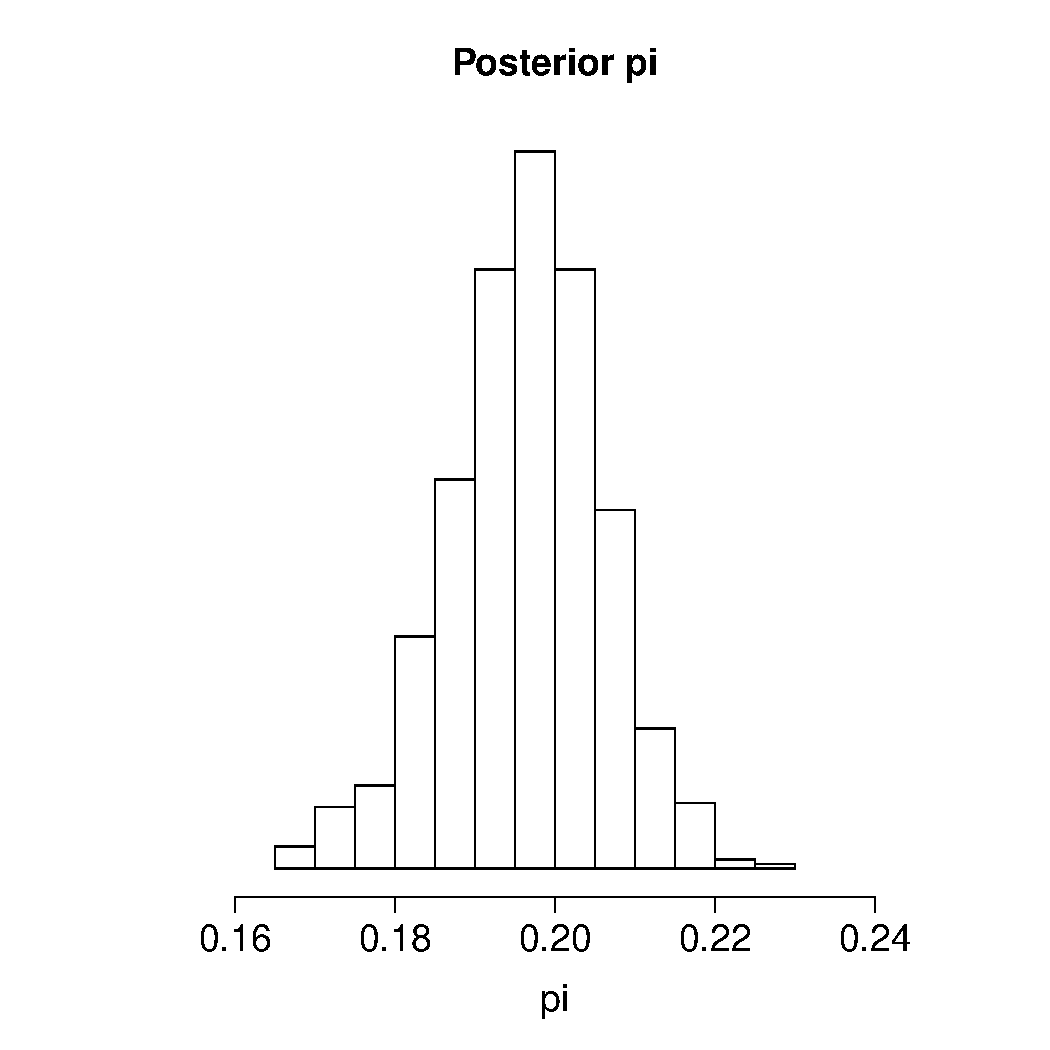
\includegraphics[height=0.6\textheight]{pdf/dentistry-prevalence.pdf}



\sld{Posteriors for Dentist Accuracies}

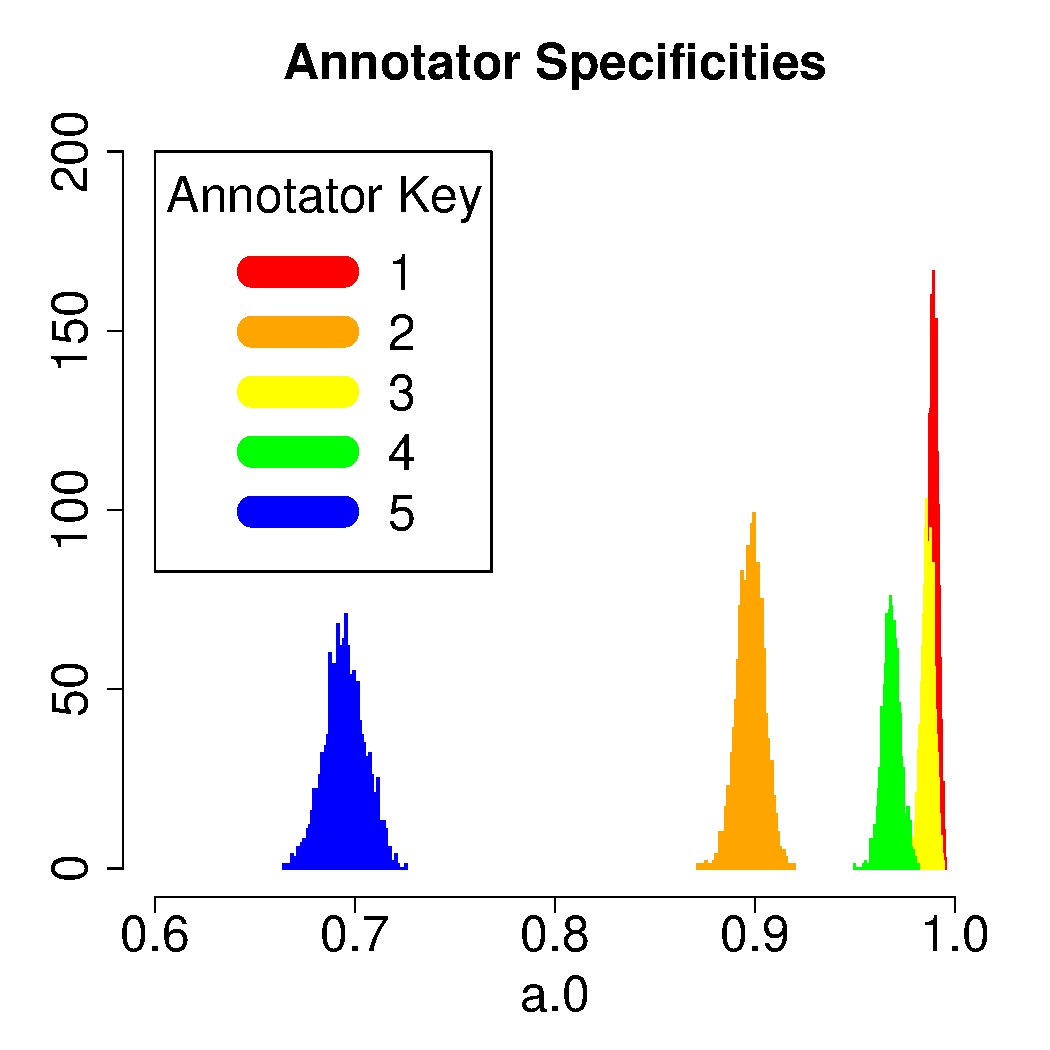
\includegraphics[width=0.4\textwidth]{pngs/a-0-hist.pdf}
\ \ \
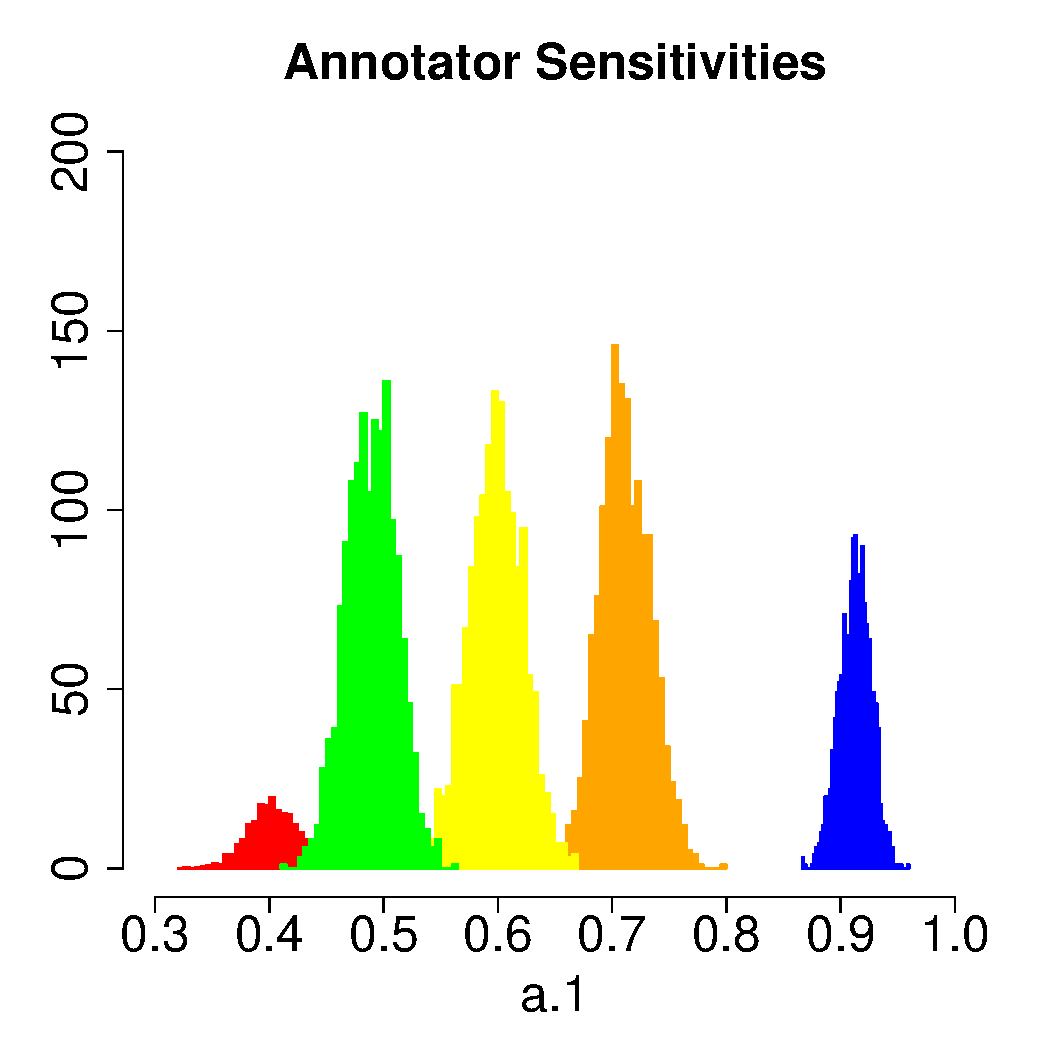
\includegraphics[width=0.4\textwidth]{pngs/a-1-hist.pdf}

\begin{itemize}
\item Posterior densities useful for downstream inference
\item Mitigates overcertainty of point estimates
\end{itemize}


\sld{Posteriors for Dentistry Data Items}

\hspace*{-24pt}
\begin{tabular}{ll}
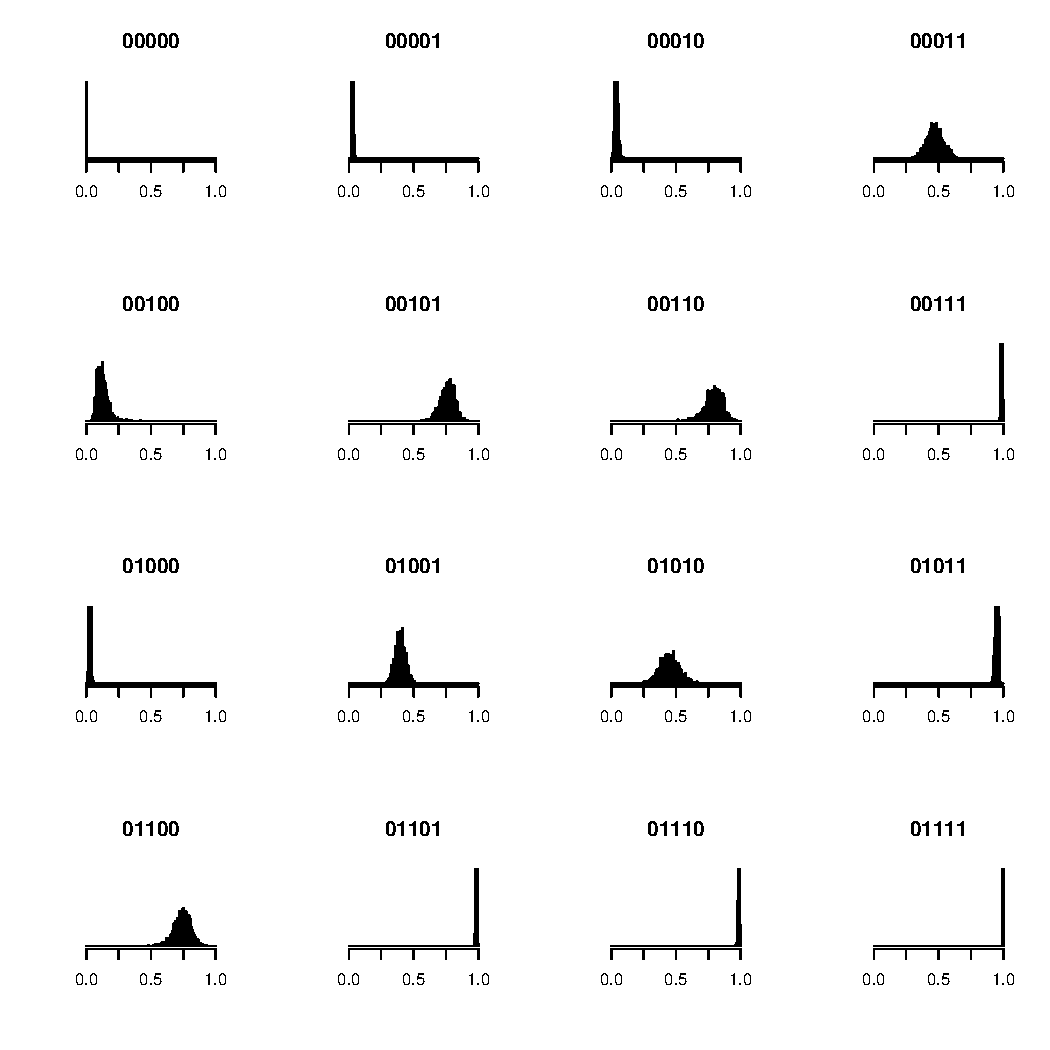
\includegraphics[width=0.5\textwidth]{pngs/model-4-cat-posteriors-dentistry.pdf}
&
\includegraphics[width=0.5\textwidth]{pngs/model-4-cat-posteriors-dentistry-2.pdf}
\end{tabular}
\vspace*{-4pt}
\begin{itemize}
\footnotesize
\item Accuracy adjustment results are very different than simple vote
\end{itemize}

\sld{Marginal Evaluation}
{\footnotesize
\begin{itemize}
\item Common evaluation in epidemiology uses $\chi^2$ on marginals
\\[12pt]
\begin{tabular}{rr|rrr}
{\it Positive} &   & \multicolumn{3}{c}{{\it Posterior Quantiles}} \\
{\it Tests} & {\it Frequency} & {\it .025} & {\it .5} & {\it .975} \\  \hline
0 & 1880 & 1818 & 1877 & 1935 \\
1 & 1065 & 1029 & 1068 & 1117 \\
2 & 404 & 385 & 408 & 434 \\
3 & 247 & 206 & 227 & 248 \\
4 & 173 & 175 & 193 & 212 \\
5 & 100 & 80 & 93 & 109 \\
\end{tabular}
\\[8pt]
\item Simpler models (all accuracies equal) are underdispersed (not enough all-0 or all-1 results)
\item Better marginal eval is over all items (e.g. 00100, 01101, \ldots)
\item Accounting for item difficulty provides even tighter fit
\end{itemize}
}


\mypart{Applications}

\sld{Is the Truth Out There?}
\begin{itemize}
\item Or are the ``gold standards'' just fool's gold?
\item Evaluate uncertainty in item category with $\mbox{\rm Pr}(c_i = 1)$
\item Do all items even have true categories?
\begin{itemize}
\footnotesize
\item Coding standard may be vague (e.g. ``Mars'' as location [MUC-6])
\item Distinguishing author/speaker intent from interpretation
\end{itemize}
\item Items often don't have clear interpretation
\begin{itemize}
\footnotesize
\item Some items hard to distinguish categorically (esp. metonymy)
\item e.g. ``New York'' as team or location or political entity
\item e.g. ``p53'' as gene/protein, wild/mutant, human/mouse
\end{itemize}
\end{itemize}

\sld{Evaluating Annotators}
\begin{itemize}
\item Not all annotators have the same accuracy
\item Ideally, annotators have high sensitivity and specificity
\item Ideally annotators are unbiased 
\begin{itemize}
\footnotesize
\item Bias indicated by sensitivity $>>$ specificity or vice-versa
\end{itemize}
\item Provide feedback to help annotators improve
\item Filter annotators to contribute to coding
\item Deciding how many annotators needed for an item
\end{itemize}

\sld{Evaluating ``Gold'' Labels}
\begin{itemize}
\item Get probabilities $\mbox{\rm Pr}(c_i=1)$
\item Middling probabilities mean annotators uncertain
\item Find items for which annotators having difficulty
\begin{itemize}
\footnotesize
\item Refine coding standard by adjudicating examples
\end{itemize}
\item (Alternative to explicitly modeling item difficulty)
\end{itemize}

\sld{Speed versus Accuracy}
\begin{itemize}
\item Assume all we have goal for ``gold standard'' accuracy
\item May be beneficial to trade accuracy for speed
\begin{itemize}
\footnotesize
\item e.g. 150 items at 80\% accuracy vs.\ 100 items at 90\%
\item Former may be better with voting with adjustment for accuracies
\end{itemize}
\item Less-than-perfect gold standard acceptable for some tasks
\begin{itemize}
\footnotesize
\item Many machine learning procedures robust to noise
\item More problematic for evaluating ``state of the art''
\end{itemize}
\end{itemize}

\sld{New Items versus New Labels}
\begin{itemize}
\item Evaluate whether to generate
\begin{itemize}
\footnotesize
\item A new label for an uncertainly labeled item, or
\item a new label for currently unlabeled item
\item (Sheng, Provost and Ipeirotis 2009)
\end{itemize}
\item Choose which annotator to label item
\begin{itemize}
\footnotesize
\item Can measure expected gain in certainty given annotator accuracy
\item Like active learning, only for annotators rather than items
\end{itemize}
\end{itemize}


\sld{Evaluating Coding Standard Difficulty}
\begin{itemize}
\item Replacement for $\kappa$ with predictive power for new annotators
\item Allows inference on correctness of gold standard
\item Sensitivity and Specificity priors $(\alpha,\beta)$ model:
\begin{itemize}
\footnotesize
\item Mean annotator accuracy
\item Annotator variation
\item Annotator bias
\end{itemize}
\item Low mean accuracy indicates a problematic coding standard
\end{itemize}

\sld{Probabilistic Training and Testing}
\begin{itemize}
\item Use probabilistic item posteriors for training
\begin{itemize}
\footnotesize
\item Easy to generalize most probabilistic models 
\item e.g. naive Bayes or HMMs: \ proportional train (as for EM)
\item e.g. logistic regression or CRFs: \ modify log loss
\item Generalize arbitrary model with posterior samples (e.g. SVMs)
\end{itemize}
\item Use probabilistic item posteriors for testing
\begin{itemize}
\footnotesize
\item Penalizes overconfidence of models on uncertain items
\item Easy generalization with log loss evaluation
\item Not so clear with first-best accuracy or F-measure
\end{itemize}
\item Demonstrated theoretical effectiveness (Smyth 1995)
\end{itemize}


\sld{Bayesian {\Large $\kappa$} Estimates}
\begin{itemize}
\item Given estimated sensitivity, specificity and prevalence:
\begin{itemize}
\footnotesize
\item Calculate expected $\kappa$ for two annotators
\item Don't even need to annotate common items
\item Calculate expected $\kappa$ for two new annotators
\item Calcluate confidence/posterior uncertainty of $\kappa$
\item May formulate hypothesis tests
\item e.g. $\kappa$ for given standard above 0.8
\item e.g. $\kappa$ for coding standard 1 higher than for standard 2
\end{itemize}
\item Always a good idea to measure posterior uncertainty
\item May estimate Bayesian posteriors (or frequentist confidence intervals) without annotation model
\end{itemize}



\mypart{Hierarchical Bayesian \\[12pt]\hspace*{12pt}Annotation Model}
\vfill
(Carpenter 2008)

\sld{Generative Annotation Model Sketch}

\begin{picture}(195,145)

\gmnode{57.5}{132.5}{\alpha_0}
\gmnode{97.5}{132.5}{\beta_0}
\gmnode{142.5}{132.5}{\alpha_1}
\gmnode{182.5}{132.5}{\beta_1}
\gmnode{77.5}{92.5}{\theta_{0,j}}
\gmnode{162.5}{92.5}{\theta_{1,j}}
\gmnode{10}{30}{\pi}
\gmnode{55}{30}{c_i}
\gmnode{120}{30}{x_k}

\put(57.5,122.5){\vector(1,-1){19.75}}  % alpha_0 to theta_0_j
\put(97.5,122.5){\vector(-1,-1){19.75}} % beta_0 to theta_0_j
\put(142.5,122.5){\vector(1,-1){19.75}}  % alpha_1 to theta_1_j
\put(182.5,122.5){\vector(-1,-1){19.75}} % beta_1 to theta_1_j
\put(20,30){\vector(1,0){25}}  % \pi to c_i
\put(65,30){\vector(1,0){45}}  % c_i to x_k
\put(77.5,82.5){\vector(1,-1){42.5}}  % theta_0_j to x_k
\put(162.5,82.5){\vector(-1,-1){42.5}}  % theta_1_j to x_k

\gmplate{30}{55}{50}{50}{I}
\gmplate{95}{55}{50}{50}{K}
\gmplate{45}{115}{150}{45}{J}

\end{picture}

\sld{Generative Model of Annotation Process}
\begin{itemize}
\footnotesize
\item Models \underline{all} random variables given constant (hyper)priors
\item Annotators don't all label all items
\item Label $x_k$ by annotator $i_k$ for item $j_k$
\end{itemize}
{\footnotesize
\vspace*{-2pt}
\begin{eqnarray*}
\pi & \sim & \mathsf{Beta}(1,1) = \mathsf{Unif}([0,1])
\\
c_i & \sim & \mathsf{Bernoulli}(\pi)
\\
\theta_{0,j} & \sim & \mathsf{Beta}(\alpha_0,\beta_0)
\\
\theta_{1,j} & \sim & \mathsf{Beta}(\alpha_1,\beta_1)
\\
x_k & \sim & \mathsf{Bernoulli}(c_{i_k} \theta_{1,j_k}
                                        + (1 - c_{i_k}) (1 - \theta_{0,j_k}))
\end{eqnarray*}}
\begin{itemize}
\footnotesize
\item Same annotation model as before for labels $x$ 
given accuracies $\theta$ and category $c$
\item Additionally model generation of prevalence $\pi$, 
categories $c$, and accuracies $\theta$
\end{itemize}

\sld{Hierarchical Generation of Hyperpriors}
\begin{itemize}
\footnotesize
\item Models annotator population: mean accuracies and variability
\item Infers appropriate smoothing for low counts
\item Prior mean accuracy: \ $\alpha/(\alpha+\beta)$
\item Prior mean scale (inverse variability): \ $(\alpha+\beta)$
\vspace*{4pt}
{\footnotesize
\begin{eqnarray*}
\alpha_0/(\alpha_0 + \beta_0) & \sim & \mathsf{Beta}(1,1)
\\
\alpha_0 + \beta_0 & \sim & \mathsf{Pareto}(1.5)
\\
\alpha_1/(\alpha_1 + \beta_1) & \sim & \mathsf{Beta}(1,1)
\\
\alpha_1 + \beta_1 & \sim & \mathsf{Pareto}(1.5)
\end{eqnarray*}}
\item $\mathsf{Beta}(1,1)$ uniform prior on mean accuracies $\alpha/(\alpha+\beta) \in [0,1]$
\item $\mathsf{Pareto}(x|1.5) \propto x^{-2.5}$ a diffuse prior for scales $\alpha+\beta \in [0,\infty)$
\end{itemize}

\sld{Sampling Notation Defines Joint Density}
\footnotesize
\vspace*{4pt}\hspace*{12pt}
$\begin{array}{l}
p(c,x,\theta_0,\theta_1,\pi,\alpha_0,\beta_0,\alpha_1,\beta_1)
\\[4pt]
{} \ \ \ {} = \prod_{i=1}^I \mathsf{Bern}(c_i|\pi)
\\[4pt]
{} \ \ \ \ \ \ \ {} \times \prod_{k=1}^K \mathsf{Bern}(x_k|c_{i_k} \theta_{1,j_k}
                                        + (1 - c_{i_k}) (1 - \theta_{0,j_k}))
\\[4pt]
{} \ \ \ \ \ \ \ {} \times \prod_{j=1}^J \mathsf{Beta}(\theta_{0,j}|\alpha_0,\beta_0)
\\[4pt]
{} \ \ \ \ \ \ \ {} \times \prod_{j=1}^J \mathsf{Beta}(\theta_{1,j}|\alpha_1,\beta_1)
\\[4pt]
{} \ \ \ \ \ \ \ {} \times \mathsf{Beta}(\pi|1,1)
\\[4pt]
{} \ \ \ \ \ \ \ {} \times \mathsf{Beta}(\alpha_0/(\alpha_0+\beta_0)|1,1)
\\[4pt]
{} \ \ \ \ \ \ \ {} \times \mathsf{Beta}(\alpha_1/(\alpha_1+\beta_1)|1,1)
\\[4pt]
{} \ \ \ \ \ \ \ {} \times \mathsf{Pareto}(\alpha_0+\beta_0|1.5)
\\[4pt]
{} \ \ \ \ \ \ \ {} \times \mathsf{Pareto}(\alpha_1+\beta_1|1.5)
\end{array}$
\begin{itemize}
\footnotesize
\item Marginals: \ $p(x) = \int p(x,y) \ dy$; \ \ Conditionals: \ $p(y|x) = p(x,y)/p(x)$
\end{itemize}


\mypart{Gibbs Sampling}

\sld{Gibbs Sampling}
\begin{itemize}
\item General purpose Markov Chain Monte Carlo (MCMC) method
\begin{itemize}
\footnotesize
\item States of Markov chain are samples of all variables
\\[4pt] e.g.
$(c^{(n)}, x^{(n)}, \theta_0^{(n)}, \theta_1^{(n)}, \pi^{(n)}, \alpha_0^{(n)}, \beta_0^{(n)}, \alpha_1^{(n)}, \beta_1^{(n)})$ 
\item It's a continuous Markov process, unlike n-gram LMs or HMMs
\end{itemize}
\item Typically randomly initialize with ``reasonable'' values
\item Next state samples each var given current value of other vars
\item Reduces sampling of joint model to conditionals
\begin{itemize}
\item Requires sampler for each variable given all others
\item We explicitly calculated $p(c_i|x,\pi,\theta_0,\theta_1)$ as example
\end{itemize}
\end{itemize}

\sld{Gibbs Sampling (cont.)}
\begin{itemize}
\item Works for any model where dependencies form directed acyclic graph
\begin{itemize}
\footnotesize
\item Such models called ``directed graphical models''
\item Variables with no priors are hyperparameters
\item All otehr variables inferred
\end{itemize}
\item BUGS automatically computes all conditional distributions
\item Convergences to stationary process sampling from posterior
\begin{itemize}
\item Typically sample from multiple chains to monitor convergence
\item Typically throw away initial samples before convergence
\end{itemize}
\item Robust compared to Expectation Maximization [EM]
\end{itemize}

\sld{Gibbs Sample Traceplots}
\begin{itemize}
\item Plots multiple chains overlaid with different colors (3 chains here)
\\
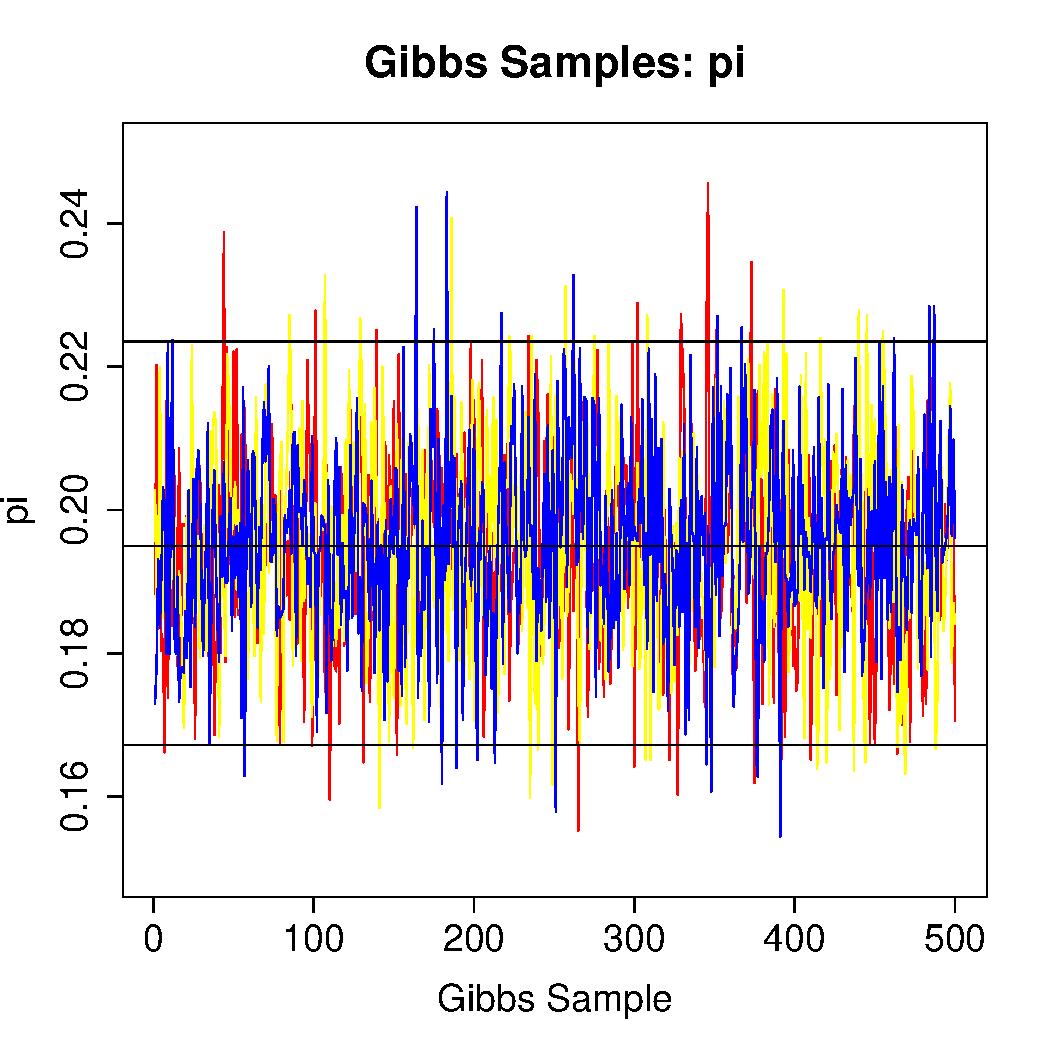
\includegraphics[height=0.5\textheight]{pdf/binomial-traceplot-pi.pdf}
\item Want to see this kind of mixing of different chains
\item Potential scale reduction statistic $\hat{R}$ characterizes mixing
\item BUGS shows traceplots for all vars; Coda package in R calcs $\hat{R}$
\end{itemize}

\sld{Gibbs Samples for Bayesian Estimation}
\begin{itemize}
\item Bayesian parameter estimate for variable $\phi$ given $N$ samples $\phi^{(n)}$
\item Approximate by averaging over collection of Gibbs samples
\\[8pt]
$\begin{array}{rcl}
\hat{\phi} 
& = & \mathbb{E}[\phi]
\\[8pt]
& = & \int \phi \ p(\phi) \ d\phi
\\[8pt]
& \approx & \frac{1}{N} \ \sum_{n=1}^N \phi^{(n)}
\end{array}$
\vspace*{4pt}
\item Provides unbiased estimate (equal to expected parameter value)
\item Works for any marginal or joint distribution of parameters
\end{itemize}


\sld{Gibbs Samples For Inference}
\begin{itemize}
\item Samples $\phi^{(n)}$ support plug-in inference
\begin{itemize}
\item E.g. Predictive Posterior Inference
\\[4pt]
$p(\tilde{y}|y) = \int p(\tilde{y}|\phi) \ p(\phi|y) \ d\phi
\approx
\frac{1}{N} \ \sum_{n =1}^N \ p(\tilde{y}|\phi^{(n)})$
\vspace*{8pt}
\item E.g. (Multiple) Variable Comparisons
\\[4pt]
$\mbox{\rm Pr}(\theta_{0,j} > \theta_{0,j'}) \approx \frac{1}{N} \ \sum_{n=1}^N \ \mbox{\rm I}(\theta_{0,j}^{(n)} > \theta_{0,j'}^{(n)})$
\\[12pt]
$\mbox{\rm Pr}(j \mbox{ best specificity}) \approx \frac{1}{N} \ \sum_{n=1}^N \ \prod_{j' = 1}^J \mbox{\rm I}(\theta_{0,j}^{(n)} \geq \theta_{0,j'}^{(n)})$
\vspace*{8pt}
\end{itemize}
\item Latter statistic can be used to compare systems (the `E' in ``LREC'')
\item More samples provide more accurate approximations
\item Plug-in estimates like (frequentist) bootstrap estimates
\end{itemize}


\mypart{Simulation Study}

\sld{Simulated Data Tests Estimators}

\begin{itemize}
\item Simulate data (with reasonable model settings)
\item Test sampler's ability to fit
\item Simulation Parameter Values
\begin{itemize}
\footnotesize
\item $J=20$ annotators, $I=1000$ items
\item prevalence $\pi = 0.2$
\item specificity prior $(\alpha_0,\beta_0) = (40,8)$ (83\% accurate, medium var)
\item sensitivity prior $(\alpha_1,\beta_1) = (20,8)$ (72\% accurate, high var)
\item specificities $\theta_1$ generated randomly given $\alpha_1, \beta_1$
\item sensitivities $\theta_1$ generated randomly given $\alpha_1, \beta_1$
\item categories $c$ generated randomly given $\pi$
\item annotations $x$ generated randomly given $\theta_0, \theta_1, c$
\item 50\% missing annotations removed randomly
\end{itemize}
\end{itemize}

\sld{Simulated Sensitivities / Specificities}

\begin{itemize}
\item Crosshairs at prior mean
\item Realistic simulation compared to (estimated) real data
\end{itemize}

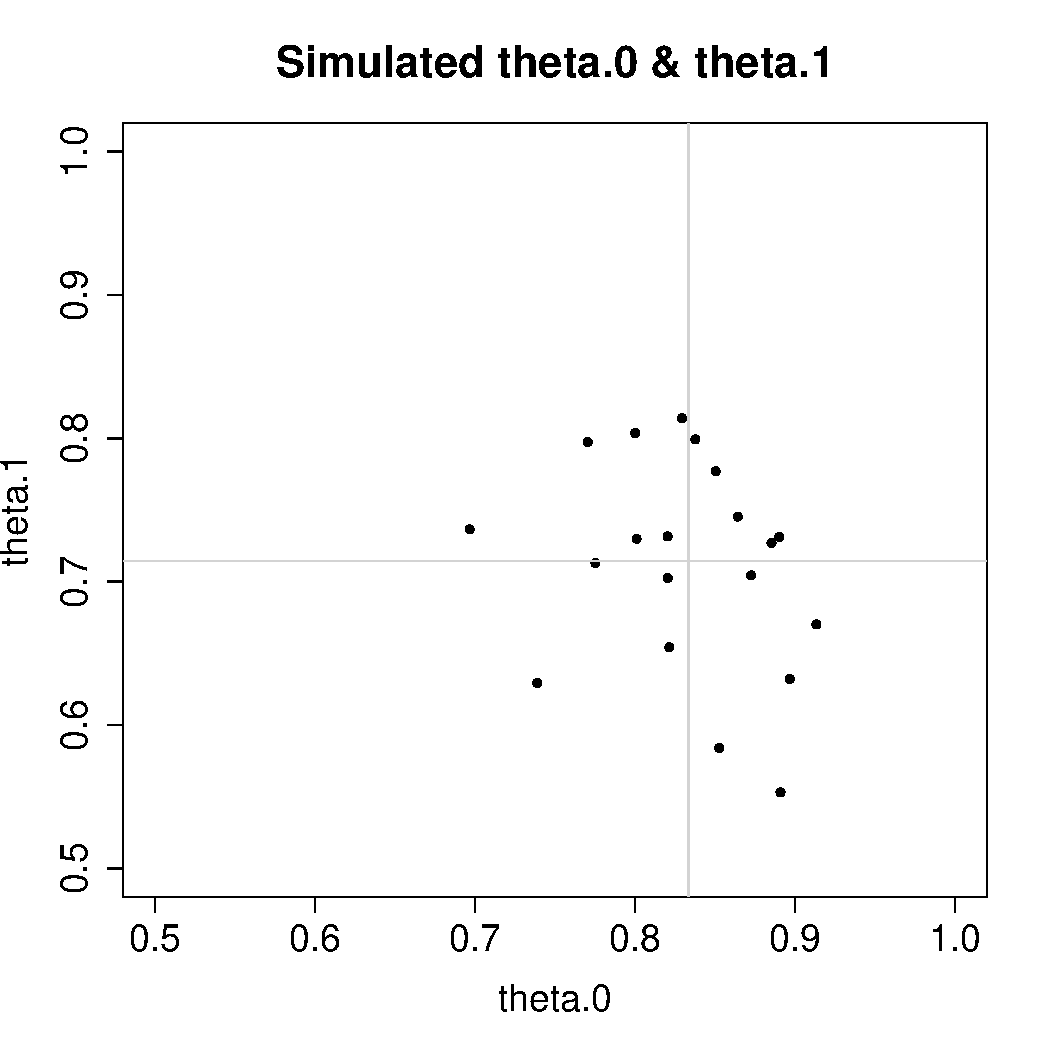
\includegraphics[width=0.4\textwidth]{pdf/beta-binomial-anno-sim-thetas.pdf}%


\sld{Prevalence Estimate}
\begin{itemize}
\footnotesize
\item Estimand of interest in sentiment (or epidemiology)
\item Simulated with prevalence $\pi = 0.2$; \ \ sample prevalence $0.21$
\item Estimates match samples; more data produces tighter estimates
\item Histogram of posterior Gibbs samples:
\end{itemize}
\hspace*{24pt}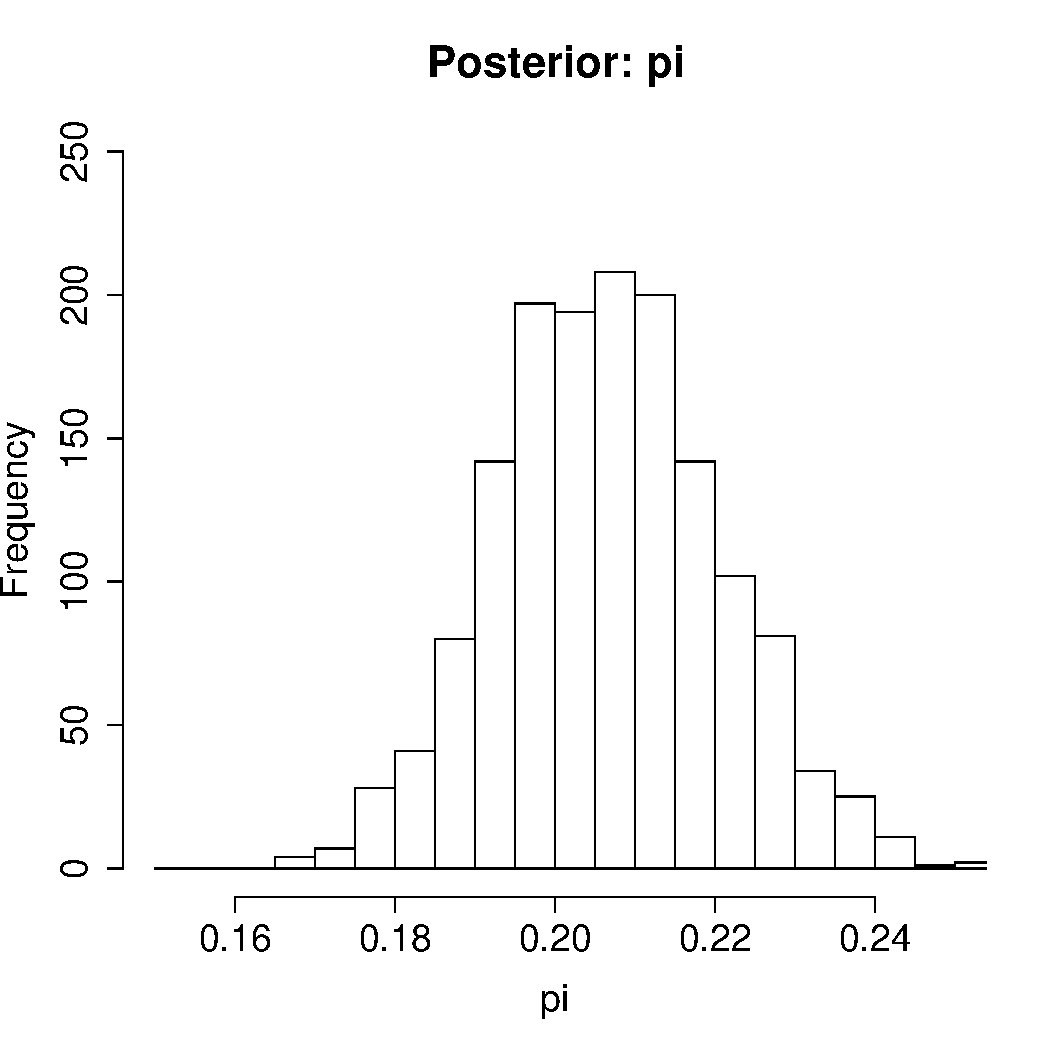
\includegraphics[width=0.35\textwidth]{pdf/beta-binomial-anno-posterior-pi.pdf}%

\sld{Sensitivity / Specificity Estimates}

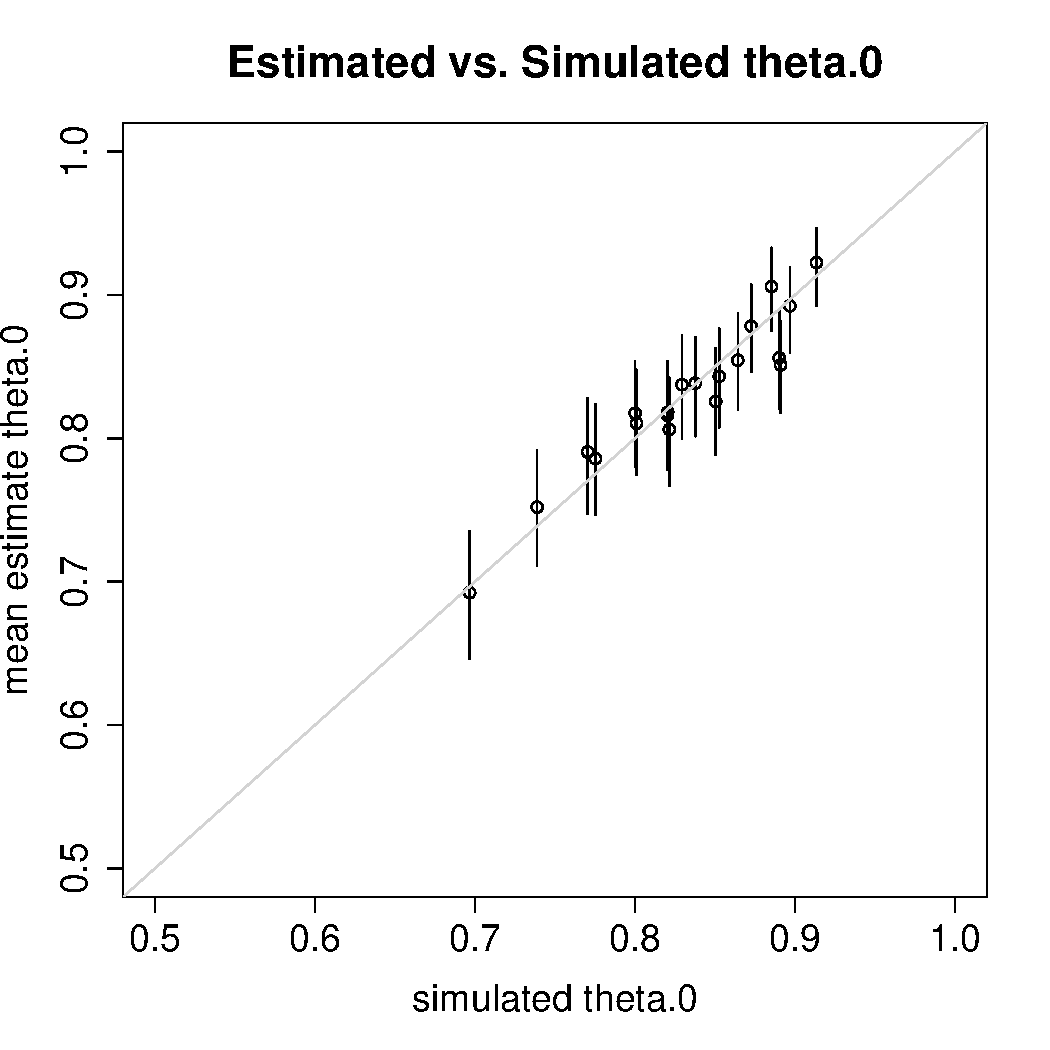
\includegraphics[width=0.4\textwidth]{pdf/beta-binomial-anno-theta0-fit.pdf}%
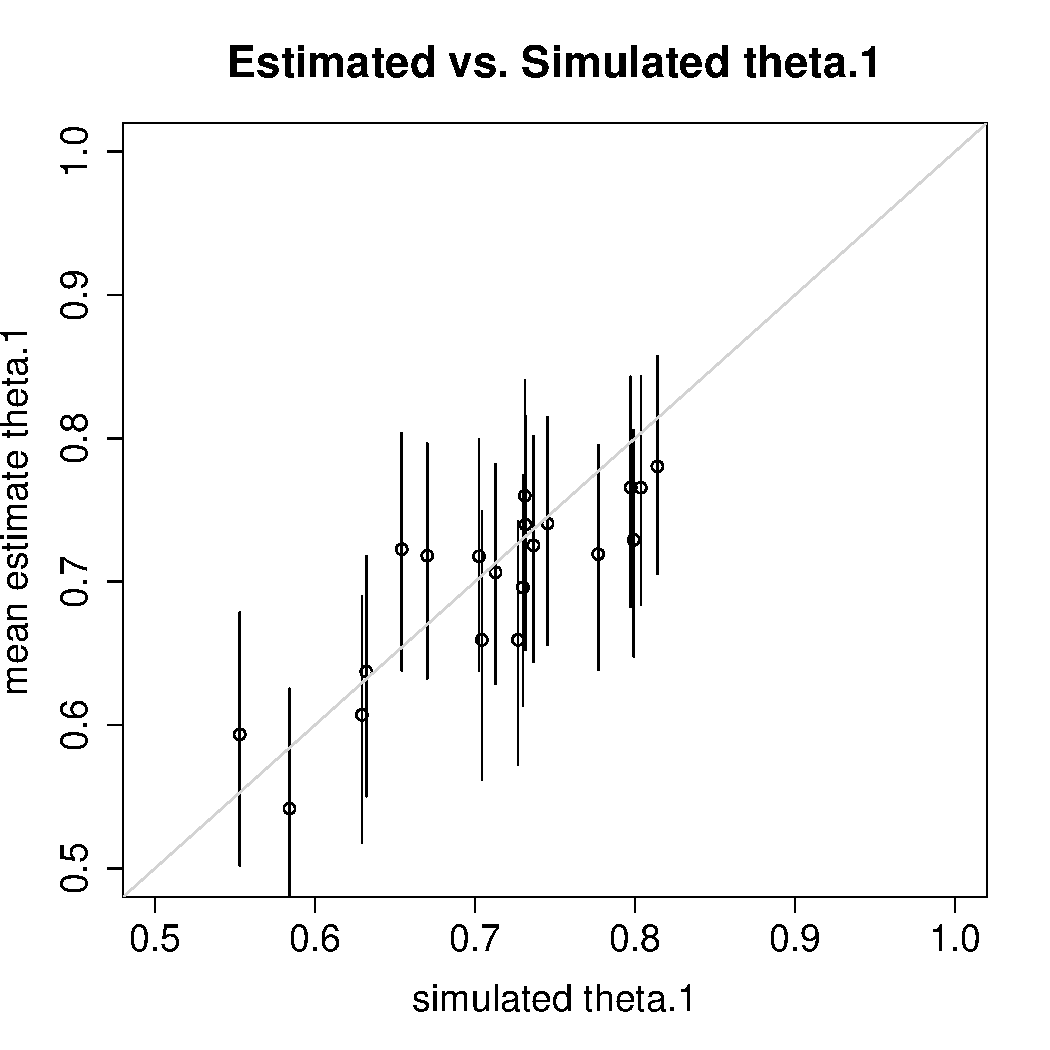
\includegraphics[width=0.4\textwidth]{pdf/beta-binomial-anno-theta1-fit.pdf}%
\vspace*{-2pt}
\begin{itemize}
\footnotesize
\item Posterior mean and 95\% intervals
\item Diagonal is perfect estimation
\item More uncertainty for sensitivity (more data w.\ $\pi = 0.2$)
\end{itemize}


\sld{Sens / Spec Hyperprior Estimates}
\vspace*{-8pt}
\begin{itemize}
\footnotesize
\item Posterior samples $(\alpha^{(n)},\beta^{(n)})$ scatterplot
\item Cross-hairs at simulated values; estimates at sample averages
\\[4pt]
\begin{tabular}{ll}
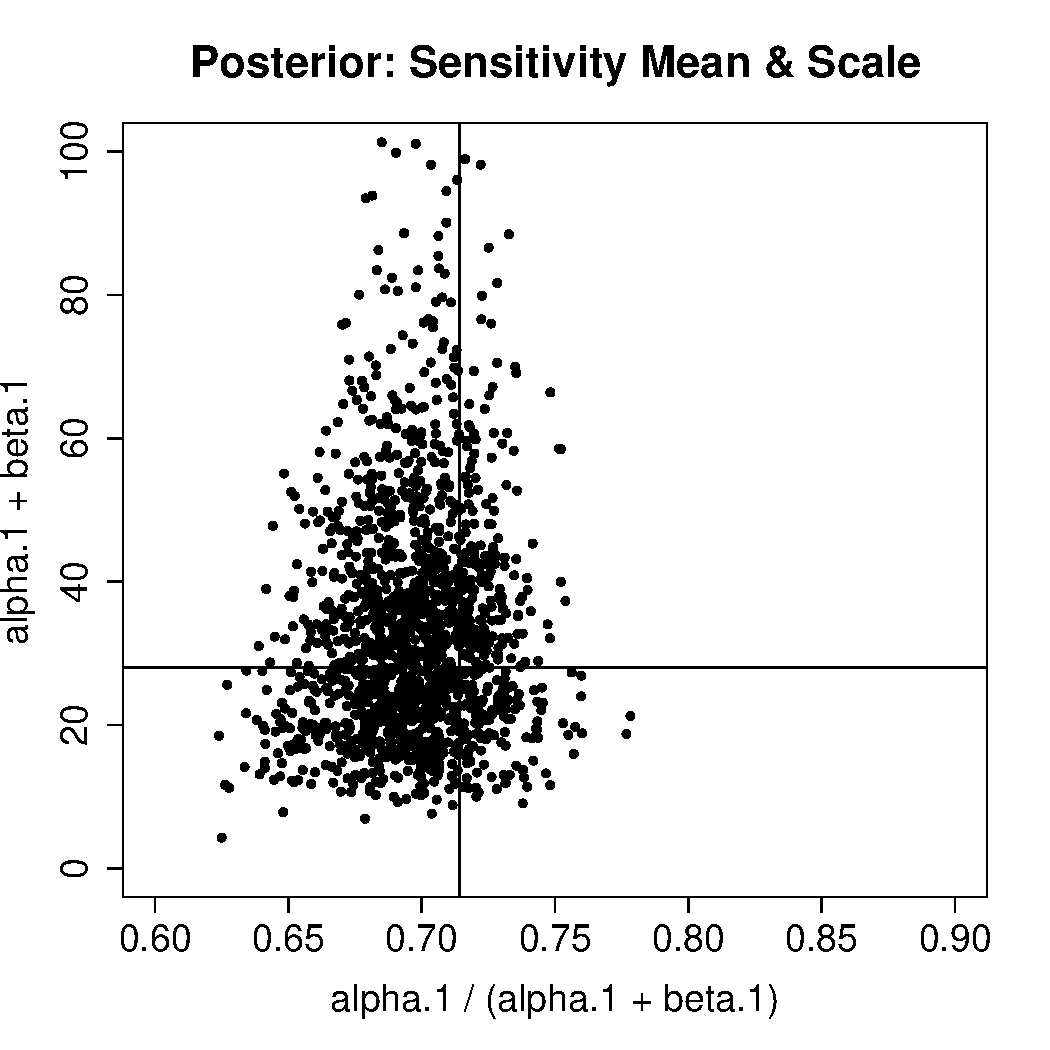
\includegraphics[width=0.40\textwidth]{pdf/beta-binomial-anno-scatter-sens.pdf}
&
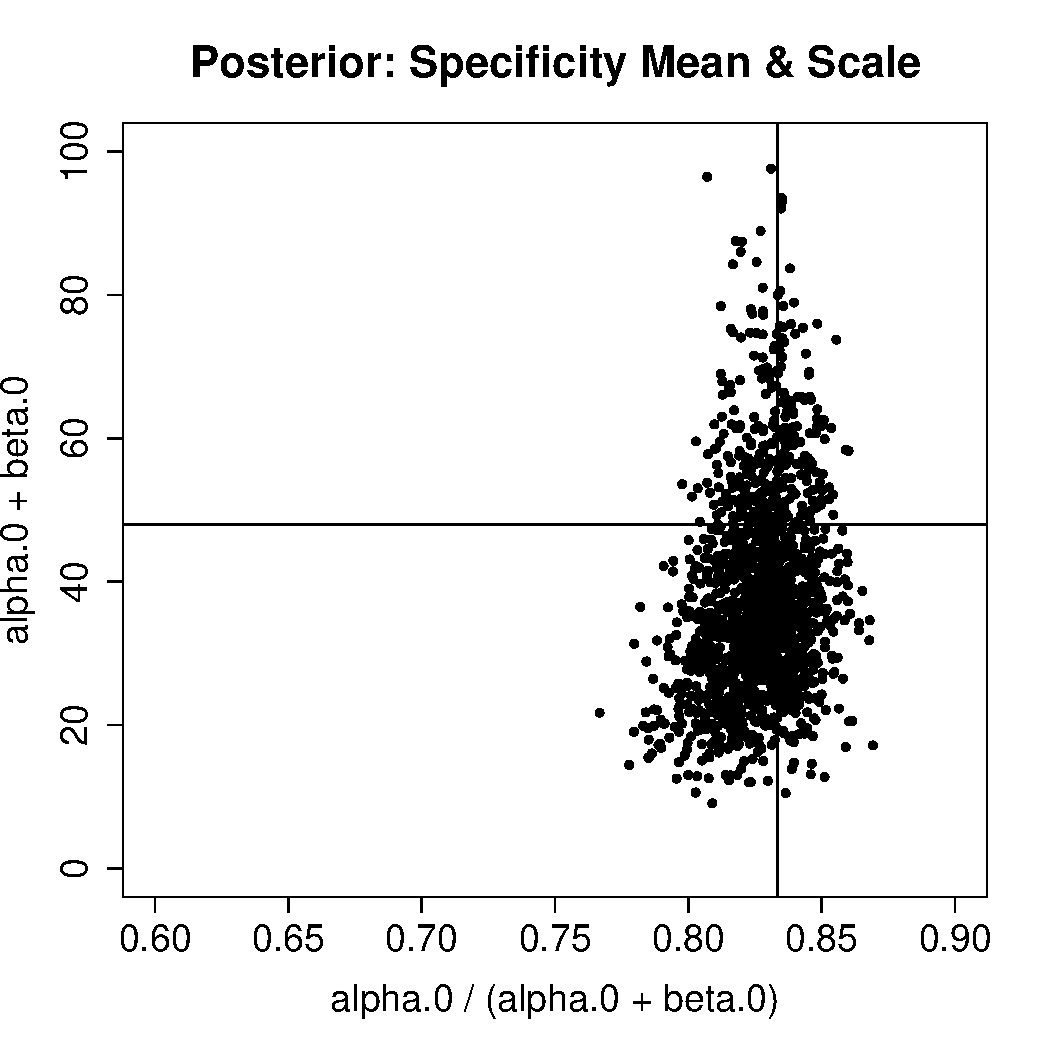
\includegraphics[width=0.40\textwidth]{pdf/beta-binomial-anno-scatter-spec.pdf}
\end{tabular}%
\item Observe typical skew to high scale (low variance)
\item More variance on sensitivity (lower counts)
\end{itemize}


\mypart{Another\\[8pt]\hspace*{8pt}Mechanical Turk Example}
\vfill
\noindent\hspace*{8pt}
(Snow, O'Connor, Jurafsky and Ng 2008)

\sld{Case 3: RTE-1}
\begin{itemize}
\item Examples and gold standard by (Dagan, Glickman and Magnini 2006)
\item 800 Items (400 true, 400 false in gold standard)
\item Examples
\begin{itemize}
\footnotesize
\item
{\it ID:} 56   \ \ \ {\it Gold Label:} TRUE
\\[2pt]
{\it Text:} Euro-Scandinavian media cheer Denmark v Sweden draw.
\\[2pt]
{\it Hypothesis:} Denmark and Sweden tie.
\\
\item
{\it ID:} 77  \ \ \ {\it Gold Label:} FALSE
\\[2pt]
{\it Text:} Clinton's new book is not big seller here.
\\[2pt]
{\it Hypotheis:} Clinton's book is a big seller.
\end{itemize}
\end{itemize}

\sld{RTE-1 Gold-Standard Procedure}
\begin{itemize}
\item Each item labeled by two annotators
\item Prevalence balanced at $\pi = 0.5$ by design
\item Censoring Data
\begin{itemize}
\footnotesize
\item Censored 20\% of data with disagreements
\item Censored another 13\% authors found ``questionable''
\item Censoring overestimates certainty and accuracy of evaluated systems on real data
\end{itemize}
\end{itemize}

\sld{RTE-1 Inter-Annotator Agreement}
\begin{itemize}
\item Inter-annotator agreement was 80\%
\item Chance agreement = $0.5^2 + 0.5^2 = 0.5$
\item $\kappa = \frac{\displaystyle 0.8 - 0.5}{\displaystyle 1 - 0.5} = 0.6$
\item Assuming 2 annotators at 80\% accuracy,
\\[4pt] expect 4\% agreement on wrong label:
\\[4pt] $(1-0.8) \times (1 - 0.8) = 0.04$
\end{itemize}

\sld{Turker Annotations for RTE-1}
\begin{itemize}
\item Collected by Dolores Labs
\item Analyzed by Snow et al. in {\it EMNLP}\ paper
\item They also recreated 4 other NLP datasets:
\begin{itemize} 
\footnotesize 
\item word sense (multinomial)
\item sentiment (multi-faceted scalar 1--100)
\item temporal ordering (binary)
\item word similarity (ordinal 1--10)
\end{itemize}
\item 2 items/task, 10 Turkers per item, 164 Turkers total
\item All five tasks completed in a few days
\item All five tasks cost under US\$100
\end{itemize}

\sld{Turker Instructions for RTE-1}
\begin{itemize}
\item Instructions
\\[6pt]
{\footnotesize Please state whether the
second sentence (the Hypothesis) is implied by the information in
first sentence (the Text), i.e., please state whether the Hypothesis
can be determined to be true given that the Text is true.

Assume that you do not know anything about the situation except what the Text itself says. 

Also, note that every part of the Hypothesis must be implied by the Text in order for it to be true.
}
\item Plus, 2 true and 2 false examples
\end{itemize}

\sld{(Munged) Turker Data for RTE-1}
\begin{verbatim}
           Item   Coder  Label   |     k    i  j  x
  -------------------------------------------------   
     1     i[1]    j[1]   x[1]   |     1    1  1  1   
     2     i[2]    j[2]   x[2]   |     2    1  2  1
     3     i[3]    j[3]   x[3]   |     3    1  3  1
     4     i[4]    j[4]   x[4]   |     4    1  4  0
                                 |
   509   i[509]  j[509]  x[509]  |   509   51  22 0
   510   i[510]  j[510]  x[510]  |   510   51  10 1
   511   i[511]  j[511]  x[511]  |   511   52   4 1
   512   i[512]  j[512]  x[512]  |   512   52   1 1
                                 |
  8000  i[8000] j[8000] x[8000]  |  8000  800 144 1
\end{verbatim}

\sld{Gold-Standard Estimation (Again)}
\begin{itemize}
\item Snow et al.\ used published gold standard as gold standard
\item Inferred categories agreed closely with gold standard
\item Snow et al.\ showed 3--5 Turkers as good as experts in most tasks
\item Ten Turkers better than pair of ``experts''
\begin{itemize}
\footnotesize
\item Turkers better matched coding standard on disagreements
\item Lots of random (spam) annotations from Turkers
\item Filtering out bad Turkers would have better ratio
\end{itemize}
\end{itemize}


\sld{BUGS Code}
\begin{center}
{\tiny
\begin{verbatim}
    model {
      pi ~ dbeta(1,1)
      for (i in 1:I) {
        c[i] ~ dbern(pi)
      }
      for (j in 1:J) {
        theta.0[j] ~ dbeta(alpha.0,beta.0) I(.4,.99)
        theta.1[j] ~ dbeta(alpha.1,beta.1) I(.4,.99)
      }
      for (k in 1:K) {
        bern[k] <- c[ii[k]] * theta.1[jj[k]]
                 + (1 - c[ii[k]]) * (1 - theta.0[jj[k]])
        xx[k] ~ dbern(bern[k])
      }
      acc.0 ~ dbeta(1,1)
      scale.0 ~ dpar(1.5,1)  I(1,100)
      alpha.0 <- acc.0 * scale.0
      beta.0 <- (1-acc.0) * scale.0
      acc.1 ~ dbeta(1,1)
      scale.1 ~ dpar(1.5,1) I(1,100)
      alpha.1 <- acc.1 * scale.1;
      beta.1 <- (1-acc.1) * scale.1
    }
\end{verbatim}
}
\end{center}

\sld{Calling BUGS from R}
\begin{center}
{\tiny
\begin{verbatim}
    library("R2WinBUGS")
    
    data <- list("I","J","K","xx","ii","jj")
    
    parameters <- c("c", "pi","theta.0","theta.1",
                    "alpha.0", "beta.0", "acc.0", "scale.0",
                    "alpha.1", "beta.1", "acc.1", "scale.1")
    
    inits <- function() {
      list(pi=runif(1,0.7,0.8),
           c=rbinom(I,1,0.5),
           acc.0 <- runif(1,0.9,0.9),
           scale.0 <- runif(1,5,5),
           acc.1 <- runif(1,0.9,0.9),
           scale.1 <- runif(1,5,5),
           theta.0=runif(J,0.9,0.9),
           theta.1=runif(J,0.9,0.9))  }
    
    anno <- bugs(data, inits, parameters,
                 "c:/carp/devguard/sandbox/hierAnno/trunk/R/bugs/beta-binomial-anno.bug",
                  n.chains=3, n.iter=500, n.thin=5,
                  bugs.directory="c:\\WinBUGS\\WinBUGS14")
\end{verbatim}
}
\end{center}

\sld{Estimated vs.\ ``Gold'' Accuracies}

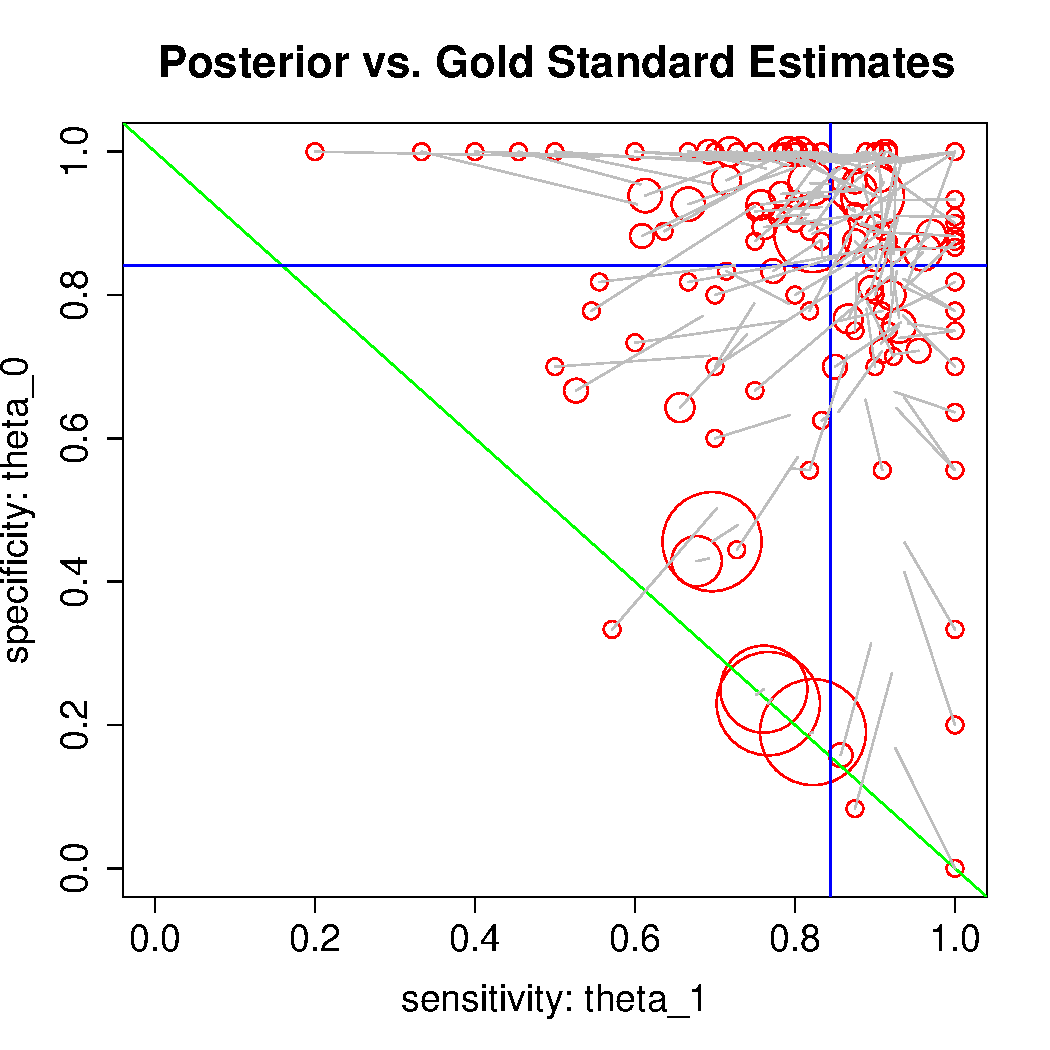
\includegraphics[width=0.4\textwidth]{pdf/dolores-rte-resids2D.pdf}%
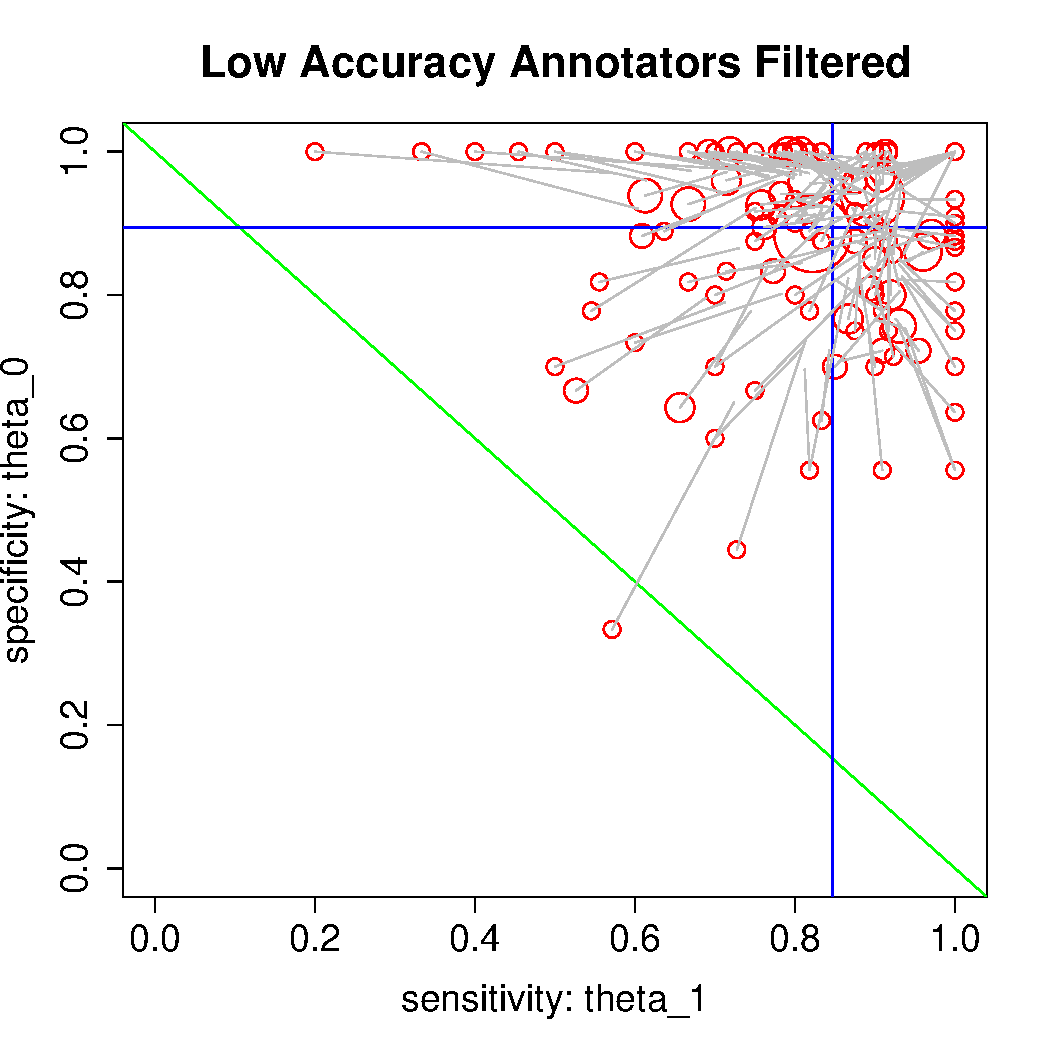
\includegraphics[width=0.4\textwidth]{pdf/dolores-rte-resids2D-pruned.pdf}%

\begin{itemize}
\footnotesize
\item Diagonal green at chance (below is adversarial)
\item  Blue lines at estimated prior means
\item Circle area is items annotated, center at ``gold standard'' accuracy, lines to estimated accuracy (note pull to prior)
\end{itemize}

\sld{Annotator Pool Estimates}
\begin{itemize}
\item Gold-standard balanced (50\% prevalence) 
\item Posterior 95\% intervals
\begin{itemize}
\footnotesize
\item Prevalence (.45,.52)
\item Specificity (.81,.87)
\item Sensitivity (.82,.87)
\item (Expect balanced sensitivity/specificity due to symmetry of task)
\end{itemize}
\item Dealing with bad Turkers
\begin{itemize}
\item 39\% of annotators no better than chance
\item more than 50\% of annotations from spammers
\item very little effect on category inference 
\item has strong effect on mean and variability of annotators
\end{itemize}
\end{itemize}


\sld{Residual Cat Errors: $c_i - \mbox{Pr}(c_i=1|\cdots$)}

\vspace*{-8pt}
\noindent
\hspace*{24pt}
\includegraphics[width=0.25\textwidth]{pdf/dolores-cat-resids-model.pdf}%
\includegraphics[width=0.25\textwidth]{pdf/dolores-cat-resids-model-pruned.pdf}%
\\
\hspace*{24pt}
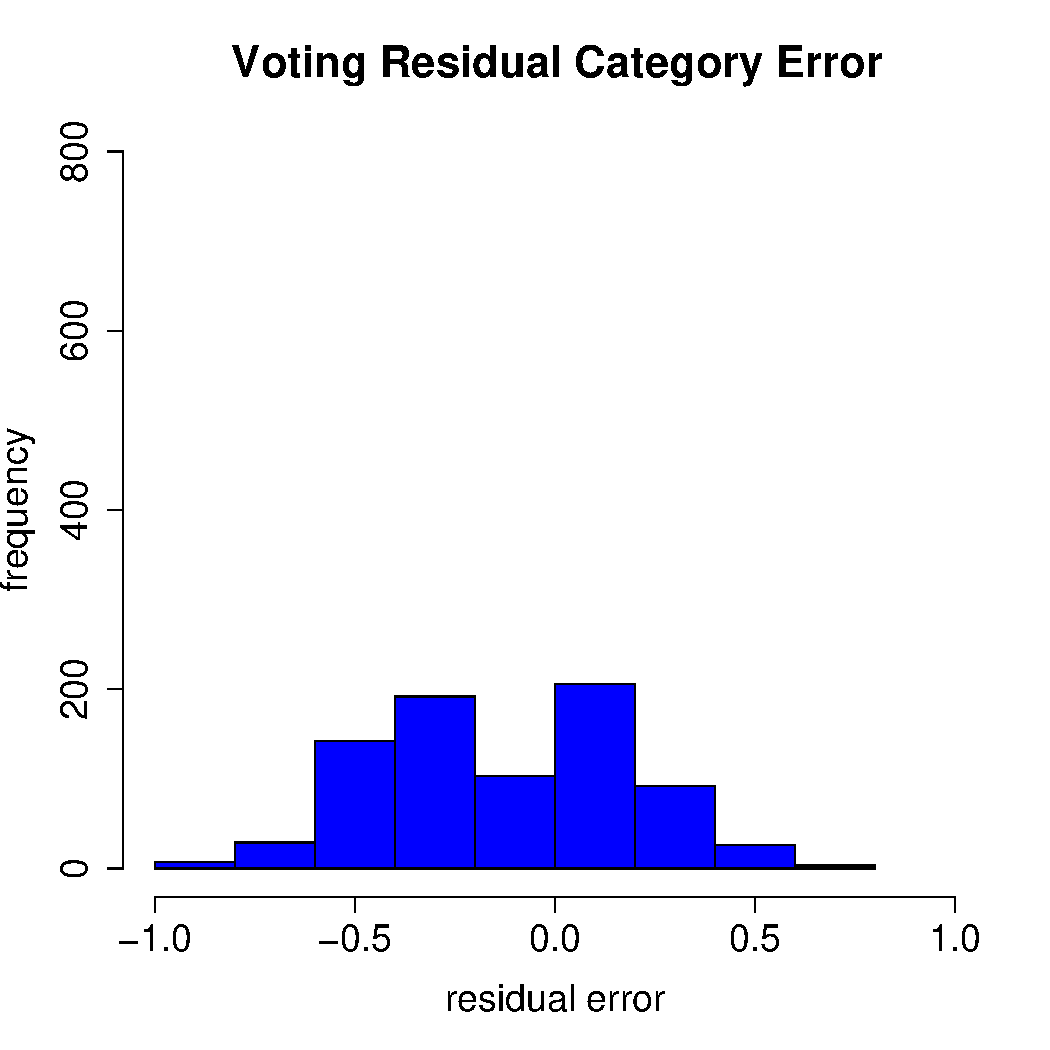
\includegraphics[width=0.25\textwidth]{pdf/dolores-cat-resids-voted.pdf}%
\includegraphics[width=0.25\textwidth]{pdf/dolores-cat-resids-voted-pruned.pdf}%
\begin{itemize}\footnotesize
\item Most residual errors in gold std (extremes of top graphs), not Turkers
\item Pruning bad annotators improves voting more than model estimates
\end{itemize}


\mypart{Modeling Item Difficulty}

\sld{Item Difficulty}

\begin{itemize}
\item Clear that some items easy and some hard
\item Assuming all same leads to suboptimal marginal fit
\item Hard to estimate even with 10 annotators/item
\begin{itemize}
\footnotesize
\item Posterior intervals too wide for good read on difficulty
\item Fattens posteriors on annotator accuracies
\item Better marginal fits (by $\chi^2$)
\end{itemize}
\item Problem is multiple explanations
\begin{itemize}
\item Good annotator accuracy, but hard items
\item Mediocre annotator accuracy, medium difficulty items
\item Poor annotator accuracy, but easy items
\end{itemize}
\end{itemize}

\sld{Mixture Item Difficulty}
\begin{itemize}
\item Assume some items easy in sense all annotators agree
\item Simple mixture model over items
\item Easy to estimate
\vfill
\item (Espeland and Handelman 1989; Beigman-Klebanov, Beigman, and Diermeier 2008)
\end{itemize}

\sld{Modeling Scalar Item Difficulty}

\begin{itemize}
\item Assume item difficulties vary on continuous scale
\item Logistic Item-Response or Rasch models
\item Used in social sciences to model educational testing and voting
\item Use logistic scale (maps $(-\infty,\infty)$ to $[0,1]$)
\item $\alpha_j$: annotator $j$'s bias (ideally 0)
\item $\delta_j$: annotator $j$'s discriminativeness (ideally $\infty$)
\item $\beta_i$: item $i$'s ``location'' (true category and difficulty)
\item $x_i \sim \mbox{logit}^{-1}(\delta_j(\alpha_i - \beta_j))$
\item Many variants of this model in epidemiology and testing
\vfill
\item (Uebersax and Grove 1993; Qu, Tan and Kutner 1996; Carpenter 2008)
\end{itemize}

\sld{Hierarchical Item Difficulty Model}

\begin{itemize}
\item Place normal (or other) priors on coefficients,
\\[4pt]
e.g. \ $\beta_i \sim \mathsf{Norm}(0,\sigma^2)$, \ \ \ $\sigma^2 \sim \mathsf{Unif}(0,100)$
\item
Priors may be estimated as before; leads to pooling of item difficulties.
\item Harder to estimate computationally in BUGS
\item Same posterior inferences when converted back to linear scale
\item e.g. average annotator accuracies, average item difficulties
\end{itemize}


\mypart{Extensions}

\sld{Extending Coding Types}
\begin{itemize}
\item Multinomial responses (Dirichlet-multinomial)
\item Ordinal responses (ordinal logistic model)
\item Scalar responses (continuos responses)
\end{itemize}

\sld{Hierarchical and Multilvel Models}
\begin{itemize}
\item Assume several coding tasks
\begin{itemize}
\footnotesize
\item e.g. multiple part-of-speech corpora 
\item e.g. multiple named-entity corpora (see Finkel and Manning 2009)
\item e.g. multiple language newswire categorization
\item e.g. coref corpora in different genres or languages
\end{itemize}
\item Estimate another level of priors 
\begin{itemize}
\footnotesize
\item e.g. for prevalence
\item e.g. for priors on accuracy priors
\end{itemize}
\item Common approach in social science models
\item Even better pooled estimates if corpora are similar
\item Multilevel models allow cross-cutting ``hierarchies''
\end{itemize}

\sld{Semi-Supervision}
\begin{itemize}
\item Easy to add in supervised cases with Bayesian models
\begin{itemize}
\footnotesize
\item Gibbs sampling skips sampling for supervised cases
\end{itemize}
\item May go half way by mixing in ``gold standard'' annotators
\begin{itemize}
\footnotesize
\item e.g. fixed values from gold standard, or
\item e.g. fixed high, but non-100\% accuracies, or
\item e.g. stronger high accuracy prior
\end{itemize}
\item With accurate supervision, improves estimates
\begin{itemize}
\item for prevalence
\item for annotator accuracies
\item for pool of annotators
\end{itemize}
\end{itemize}

\sld{Multimodal (Mixture) Priors}
\begin{itemize}
\item Model Mechanical Turk as mixture of spammers and hammers
\item This is what the Mechanical Turk data suggests
\item May also model covariance of sensitivity/specificity
\begin{itemize}
\item Use multivariate normal or T distribution 
\item with covariance matrix
\item Covariance may also be estimated hierarchically (see Lafferty and Blei 2007)
\end{itemize}
\end{itemize}

\sld{Annotator and Item Random Effects}
\begin{itemize}
\item May add random effects for annotators
\begin{itemize}
\footnotesize
\item amount of annotator training
\item number of items annotated
\item annotator native language
\item annotator field of expertise
\item intern, random undergrad, grad student, task designer
\end{itemize}
\item Also for Items
\begin{itemize}
\footnotesize
\item difficulty (already discussed)
\item type of item being annotated
\item frequency of item in a large corpus
\item capitalization in named entity detection
\end{itemize}
\item Use logistic regression with these predictors to model accuracies
\end{itemize}

\sld{Jointly Estimate Model and Annotations}
\begin{itemize}
\item Can train a model with inferred (probabilistic) gold standard
\item May use trained model like another annotator
\item May be beneficial to train multiple different annotators
\vfill
\item (Raykar, Yu, Zhao, Jerebko, Florin, Hermosillo-Valadez, Bogoni, and Moy 2009)
\end{itemize}



\mypart{Bayesian Estimation \\[12pt] \hspace*{12pt}and Inference}

\sld{Bayesian Models}
\begin{itemize}
\footnotesize
\item Observed data: \ $y$; \ \ \ Model parameter(s): \ $\phi$
\item Likelihood function (or sampling distribution): \ $p(y|\phi)$
\item Prior: \ $p(\phi)$
\item Chain rule: \ $p(y,\phi) = p(y|\phi) \ p(\phi)$
\item Marginal (prior predictive distribution): \ $p(y) = \int p(y|\phi) \ p(\phi) \ d\phi$
\item Posterior: $p(\phi|y)$ calculated via Bayes's rule
\\[4pt]
$\begin{array}{rcl}
p(\phi|y) & = & p(y,\phi) / p(y)
\\[4pt]
& = & p(y|\phi) \ p(\phi) / p(y)  
\\[4pt]
& = & p(y|\phi) \ p(\phi) / \int p(y | \phi') p(\phi') d\phi'
\\[4pt]
& \propto & p(y|\phi) \ p(\phi)
\end{array}
$
\end{itemize}

\sld{Point Estimators are ``Best'' Guesses}
\footnotesize
\begin{itemize}
\item Estimate parameters $\phi$ given observed data $y$
\item Maximum Likelihood Estimator (ML) 
\\[4pt]
$\phi^{*}(y) = \arg\max_\phi p(y|\phi)$
\\[4pt]
maximizes probability of observed data given parameters
\item Maximum a Posteriori (MAP) Estimate 
\\[4pt] 
$\hat{\phi}(y) = \arg\max_\phi p(\phi|y) = \arg\max_\phi p(y|\phi) \ p(\phi)$
\\[4pt]
maximizes probability of parameters given observed data
\item If prior is constant, [i.e. $p(\phi) = c$], then $\hat{\phi}(y) = \phi^{*}(y)$
\item Bayesian estimator (given mean square error loss) 
\\[4pt]
$\bar{\phi}(y) = \mathbb{E}[\phi] = \int \phi \ p(\phi|y) \ d\phi$
\\[4pt]
is expected parameter values given observed data
\item Bayesian estimates are unbiased by construction 
\\
{} [i.e. expected estimate is parameter's true value]
\end{itemize}

\sld{Inference}
\footnotesize
\begin{itemize}
\item Observed data $y$; \ \ New data $\tilde{y}$
\item Posterior predictive distribution: \ $p(\tilde{y}|y)$
\item Maximum likelihood approximation: \ $p(\tilde{y}|y) \approx p(\tilde{y}|\phi^*(y))$
\item MAP approximation: \ $p(\tilde{y}|y) \approx p(\tilde{y}|\hat{\phi}(y))$
\item Bayesian point approximation: \ $p(\tilde{y}|y) \approx p(\tilde{y} | \bar{\phi}(y))$
\item Bayesian posterior predictive distribution
\\[4pt]
$p(\tilde{y}|y) = \int p(\tilde{y}|\phi) \ p(\phi|y) \ d\phi$
\\[4pt]
averages over uncertainty in estimate of $\phi$ [i.e. $p(\phi|y)$]
\end{itemize}

\sld{Bernoulli Distribution (Single Binary Trial)}
\begin{itemize}
\item Outcome $y \in \{ 0, 1 \}$ \ \ [success=1, failure=0]
\item Parameter $\theta \in [0,1]$ is chance of success 
\item 
$p(y|\theta)
= \mbox{\sf Bernoulli}(y|\theta) 
= \theta^y \ (1 - \theta)^{1-y}
=
\begin{cases}
\theta & \mbox{if } $y = 1$
\\
1 - \theta & \mbox{if } $y = 0$
\end{cases}$
\vspace*{6pt}
\item
For $N$ independent trials $y = y_1,\ldots,y_N$, \ where $y_n \in \{ 0, 1 \}$,
\\[4pt]
$\begin{array}{rcl}
p(y|\theta) & = & \prod_{n = 1}^N p(y_n|\theta)
\\[4pt]
& = & \prod_{n=1}^N \theta^{y_n} \ (1-\theta)^{1-y_n}
\\[4pt]
& = & \theta^A (1-\theta)^B
\end{array}$
\\[4pt]
where $A = \sum_{n=1}^N y_n$ and $B = \sum_{n=1}^N (1 - y_n) = N - A$
\\[4pt]
\vfill
\item
{\scriptsize $x^0 = 1$ \ \ and \ \ $x^a x^b = x^{a+b}$}
\end{itemize}

\sld{Conjugate Priors}
\begin{itemize}
\item Given a sampling distribution $p(y|\phi)$
\item Given a family of distributions $\mathcal{F}$
\item The family $\mathcal{F}$ is conjugate for $p(y|\phi)$ if
\\[4pt]
prior $p(\phi) \in \mathcal{F}$ implies posterior $p(\phi|y) \in \mathcal{F}$
\item Provides analytic form of posterior (vs.\ numerical approximation)
\item Supports incremental updates
\begin{itemize}
\item Start with prior $p(\phi) \in \mathcal{F}$
\item After data $y$, have posterior $p(\phi|y) \in \mathcal{F}$
\item Use $p(\phi|y)$ as prior for new data $y'$
\item New posterior is $p(\phi|y,y') \in \mathcal{F}$
\item i.e.\ updating with $y$ then $y'$ same as upating for $y,y'$ together
\end{itemize}
\item Not necessary for Bayesian inference
\end{itemize}

\sld{Mean, Mode and Variance for Bernoulli}

\begin{itemize}
\item Mean and Mode: \ $\mathbb{E}[\mbox{\sf Bern}(\theta)] = \mbox{\rm mode}[\mbox{\sf Bern}(\theta)] = \theta$
\item Variance: \ $\mbox{\rm var}[\mbox{\sf Bern}(\theta)] = \theta \ (1-\theta)$
\item Standard Deviation: \ $\mbox{\rm sd}[\mbox{\sf Bern}(\theta)] = \sqrt{\theta \ (1-\theta)}$
\vfill
\item {\scriptsize For discrete $X$ with $N$ outcomes $x_1,\ldots,x_N$ distributed $p_X(x)$}
\begin{itemize}
\scriptsize
\item Mode (Max Value): \ $\mbox{\rm mode}[X] = \arg\max_{n=1}^N p(x_n)$
\item Mean (Average Value): \ $\mathbb{E}[X] = \sum_{n=1}^N p(x_n) \ x_n $
\item Variance: \ $\mbox{\rm var}[X] = \mathbb{E}[X-\mathbb{E}[X]] = \sum_{n=1}^N p(x_n) \ (x_n - \mathbb{E}[X])^2$
\item Standard Deviation: \ $\mbox{\rm sd}[X] = \sqrt{\mbox{\rm var}[X]}$
\end{itemize}
\end{itemize}

\sld{Beta Distribution}
\begin{itemize}
\item Outcome $\theta \in [0,1]$
\item Parameters $\alpha,\beta > 0$
\ \ \ [$\alpha-1$ prior successes; $\beta-1$ failures]
\item 
Continuous Density Function
\\[4pt]
$\begin{array}{rcl}
p(\theta|\alpha,\beta) 
& = & \mbox{\sf Beta}(\theta|\alpha,\beta)
\\[8pt]
& = & \frac{1}{\displaystyle \mbox{\rm B}(\alpha,\beta)} \ \ \theta^{\alpha-1} \ (1-\theta)^{\beta-1}
\\[8pt]
& \propto & \theta^{\alpha-1} \ (1-\theta)^{\beta-1}
\end{array}$
\vfill
\item {\scriptsize
Continuous densities $p(\theta)$ have $p(\theta) \geq 0$ and $\int p(\theta) d\theta = 1$
}
\item {\scriptsize
Beta function $\mbox{\rm B}(\alpha,\beta) = \int_0^1 \theta^{\alpha-1} \ (1-\theta)^{\beta-1} \ d\theta 
=  \frac{\Gamma(\alpha+\beta)}{\Gamma(\alpha)\Gamma(\beta)}$}
\item {\scriptsize
$\Gamma(x) = \int_0^{\infty} y^{x-1} \ \exp(-y) dy$ \ \ is continuous generalization of factorial
\\[4pt]
i.e. $\Gamma(n+1) = n! = n \times (n-1) \times \cdots\times 2 \times 1$ \ for integer $n \geq 0$}
\end{itemize}

\sld{\normalsize Beta Examples}

\vspace*{-8pt}
% 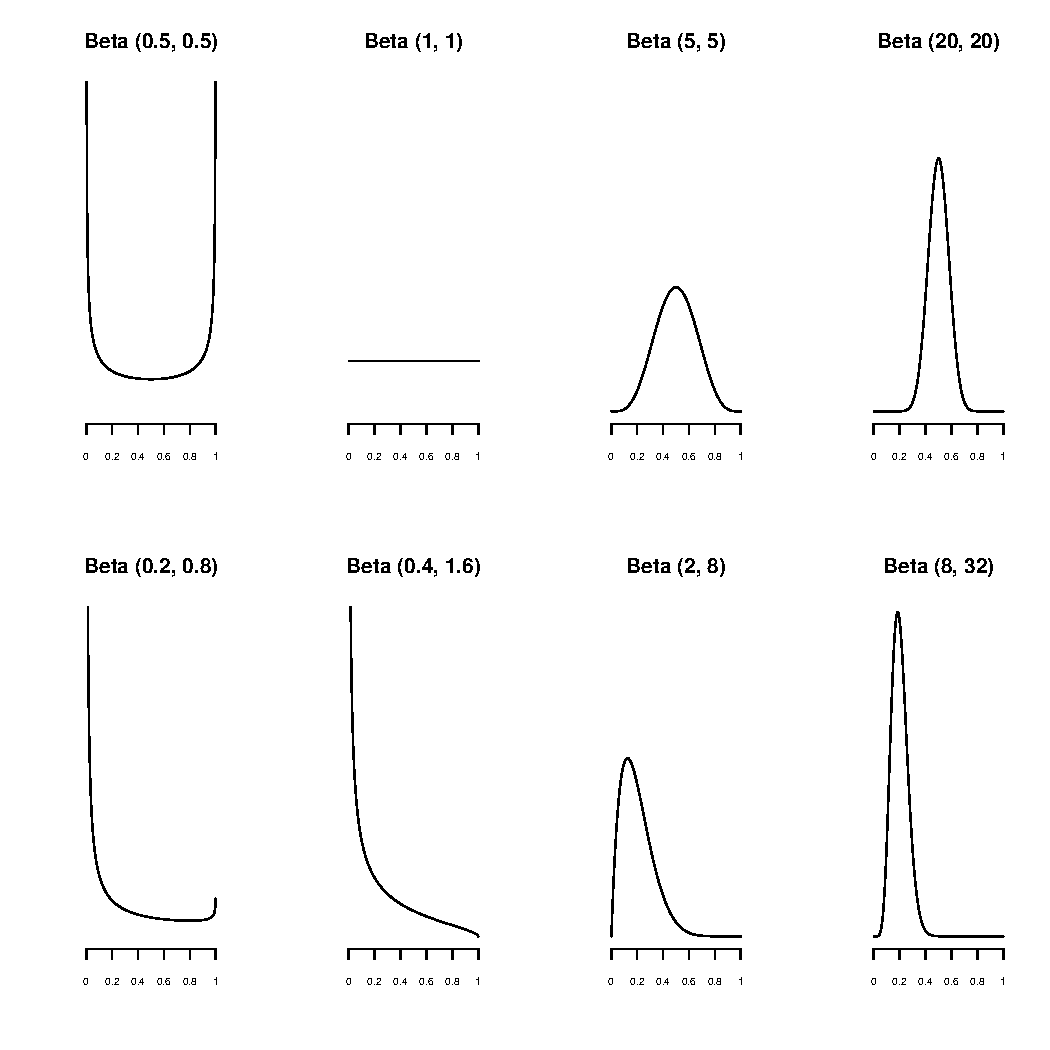
\includegraphics[width=0.65\textwidth]{pdf/beta-examples.pdf}
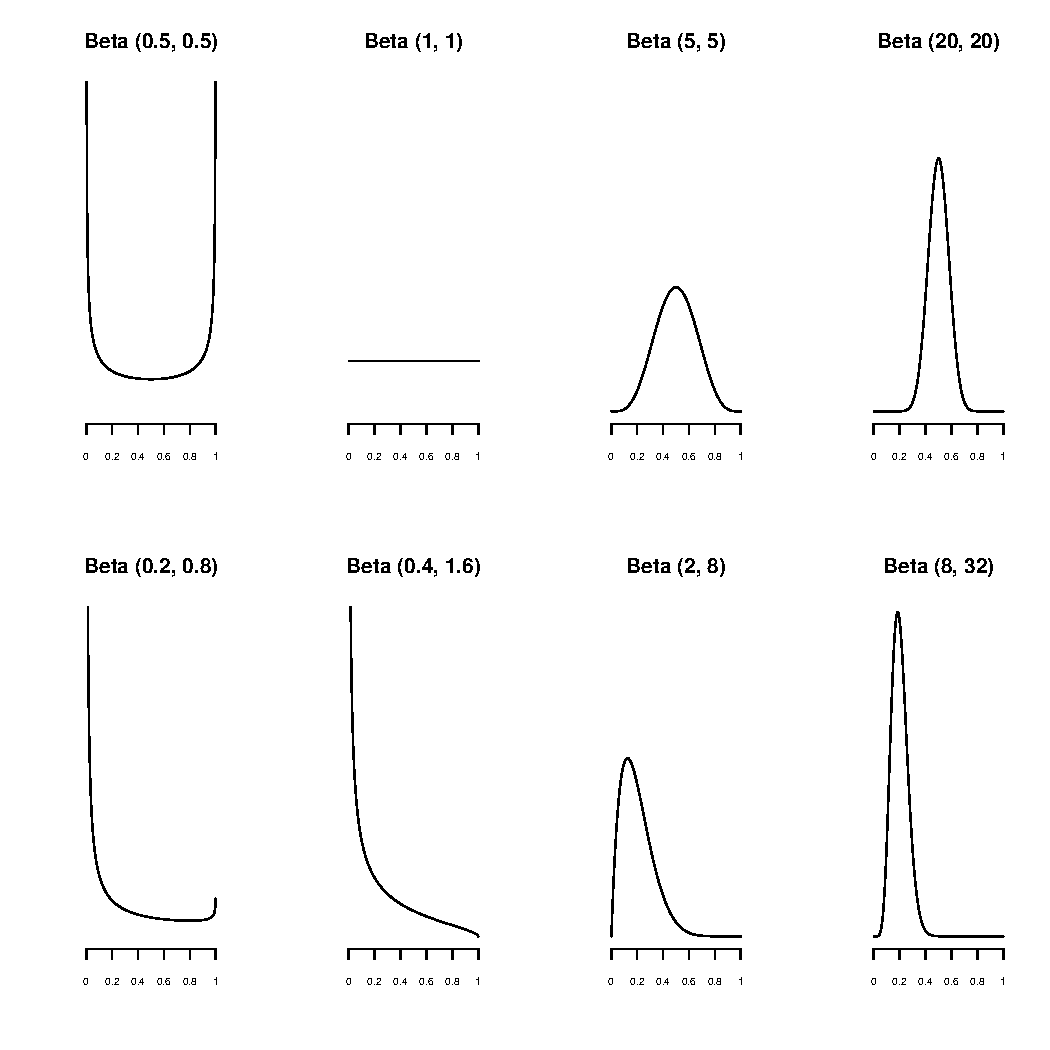
\includegraphics[height=1.0\textheight,width=0.85\textwidth]{pdf/beta-examples.pdf}


\sld{Mean, Mode and Variance for Beta}
\begin{itemize}
\item Mean: \ 
$\mathbb{E}[\mbox{\sf Beta}(\alpha,\beta)] = \frac{\displaystyle \alpha}{\displaystyle \alpha+\beta}$
\item Variance: \ 
$\mbox{\rm var}[\mbox{\sf Beta}(\alpha,\beta)] = \frac{\displaystyle \alpha\beta}{\displaystyle (\alpha+\beta)^2 \ (\alpha + \beta + 1)}$
\item Mode: \ 
$\mbox{\rm mode}[\mbox{\sf Beta}(\alpha,\beta)] 
= 
\begin{cases} 
\frac{\displaystyle \alpha-1}{\displaystyle \alpha+\beta-2} & \mbox{if } \alpha > 1 \mbox{ and } \beta > 1
\\[4pt]
\mbox{undefined} & \mbox{otherwise}
\end{cases}$
\end{itemize}


\sld{Beta is Conjugate Prior for Bernoulli}
\begin{itemize}
\item Data is $N$ Bernoulli samples $y = y_1,\ldots,y_N$ for $y_n \in \{ 0, 1 \}$
\item Prior $p(\theta) = \mbox{\sf Beta}(\theta|\alpha,\beta)$
\item Likelihood $p(y|\theta) = \prod_{n=1}^N \mbox{\sf Bern}(y_n|\theta) = \theta^A (1-\theta)^B$
\\[4pt] {\scriptsize where $A$ is number of successes, $B$ number of failures in $y$}
\item Posterior 
\\[4pt]
$\begin{array}{rcl}
p(\theta|y) & \propto & p(y|\theta) \ p(\theta)
\\[4pt]
& = & \prod_{n=1}^N \mbox{\sf Bern}(y_n|\theta) \ \mbox{\sf Beta}(\theta|\alpha,\beta)
\\[4pt]
& \propto & \theta^A \ (1-\theta)^B \ \theta^{\alpha-1} \ (1-\theta)^{\beta-1}
\\[4pt]
& = & \theta^{A + \alpha - 1} \ (1-\theta)^{B + \beta - 1}
\\[4pt]
& \propto & \mbox{\sf Beta}(A+\alpha,B+\beta)
\end{array}$
\item i.e. add data counts $A$ and $B$ to prior counts $\alpha-1$ and $\beta-1$
\item Concrete example of incremental updates -- just addition
\end{itemize}



\mypart{The End}

\sld{References}
\begin{itemize}
\item References
\begin{itemize}
\item {\tt http://lingpipe-blog.com/}
\end{itemize}
\item Contact
\begin{itemize}
\item
{\tt carp@alias-i.com}
\end{itemize}
\item
R/BUGS (Anon) Subversion Repository
\\[4pt]
{\tt\footnotesize svn co https://aliasi.devguard.com/svn/sandbox/hierAnno}
\end{itemize}



\end{document}
